\section{Obiettivo}
L’obiettivo del lavoro svolto è stato quello di utilizzare dei Dataset di immagini biomedicali e sfruttarli per allenare una rete neurale convoluzionale il cui scopo è la classificazione. \\
Nel dettaglio, in una prima parte dell'esperienza è stato utilizzato un dataset di radiografie pettorali per addestrare un modello che riconoscesse quali tra i soggetti presentassero la polmonite e quali no. \\
Nella seconda parte si utilizza un dataset di risonanze magnetiche cerebrali per stimare una diagnosi dello stato del paziente tra 4 possibili situazioni: paziente sano, paziente con glioma, meningioma o tumore ipofisario. \\


\section{CNN per la rilevazione della polmonite}
\subsection{Il dataset}
Il dataset utilizzato,
 pubblicato sulla piattaforma Kaggle \footnote{Kaggle è una piattaforma online per competizioni di modelli predittivi e analitici fondata nel 2010. Ad oggi conta più di 500.000 utenti} da Paulo Breviglieri, è costituito da 5856 radiografie.
 É una versione rivisitata di un altro dataset le cui immagini sono state selezionate da uno studio di coorte retrospettivo \footnote{Uno studio di coorte prende in considerazione un gruppo di individui che presentano caratteristiche comuni (sesso, età, etnia…) e che hanno come unica differenza tra loro l’esposizione o meno al fattore di rischio. Questo tipo di studio identifica persone con una malattia (o altre variabili di interesse) e le paragona ad un gruppo di controllo appropriato che non presenti la patologia.

 Questo gruppo viene osservato per un periodo di tempo prestabilito, al termine del quale si analizzerà la presenza o meno dell’esito atteso.} di pazienti pediatrici di età che va da 1 a 5 anni di un centro medico di Canton (Hong Kong). Le radiografie sono state realizzate come quadro clinico di routine per i pazienti. Le immagini stesse sono state sottoposte a screening per il controllo della qualità e tutte quelle illeggibili sono state rimosse. Le diagnosi sono poi state confermate da due fisici esperti e successivamente da un terzo specialista prima di essere utilizzate per allenare sistemi di AI. \\
 Il modello di CNN utilizzato dovrà essere in grado di riconoscere i pattern di immagine tipici della malattia. L’identificazione è infatti talvolta complicata anche per i medici più esperti. \\
Sotto: esempio illustrativo di raggi-X in pazienti con polmonite. 
\begin{figure}[hb!]
\begin{subfigure}{.32\textwidth}
  \centering
  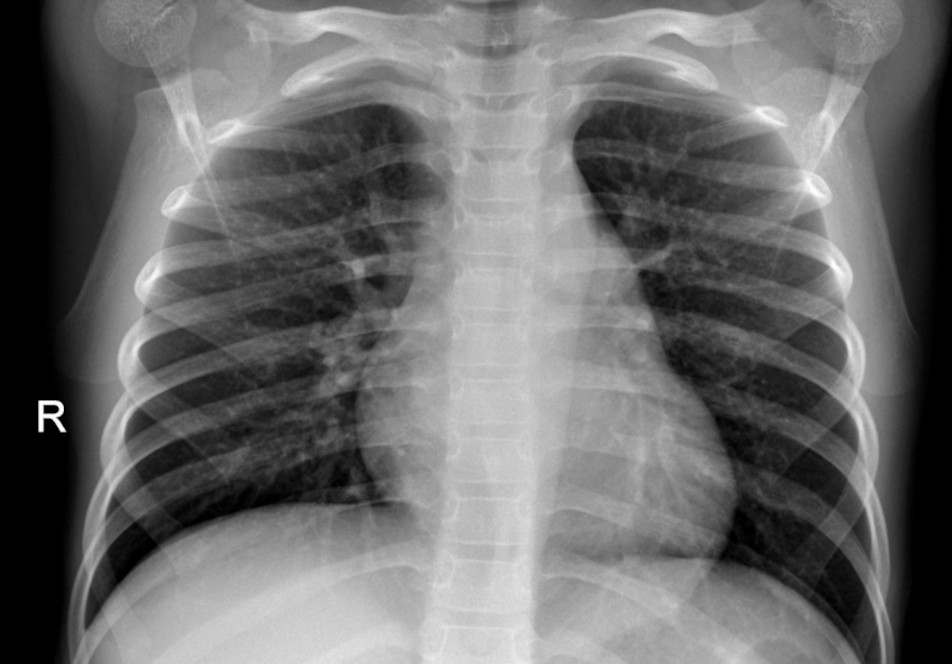
\includegraphics[width=.95\linewidth]{san}
  %\caption{1a}
  \caption{}
  \label{fig:snap1}
\end{subfigure}%
\begin{subfigure}{.32\textwidth}
  \centering
  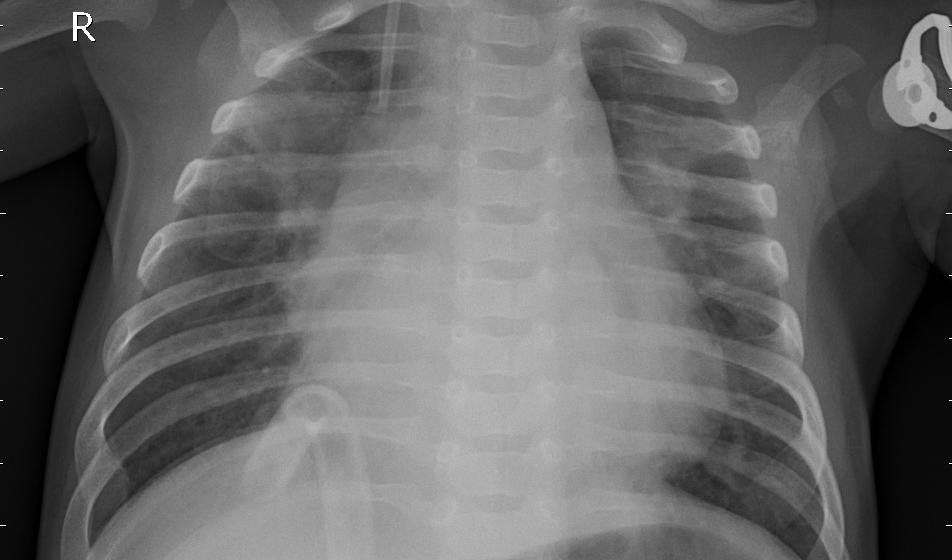
\includegraphics[width=.95\linewidth]{bacteria}
  %\caption{1a}
  \caption{}
  \label{fig:snap2}
\end{subfigure}%
\begin{subfigure}{.32\textwidth}
  \centering
  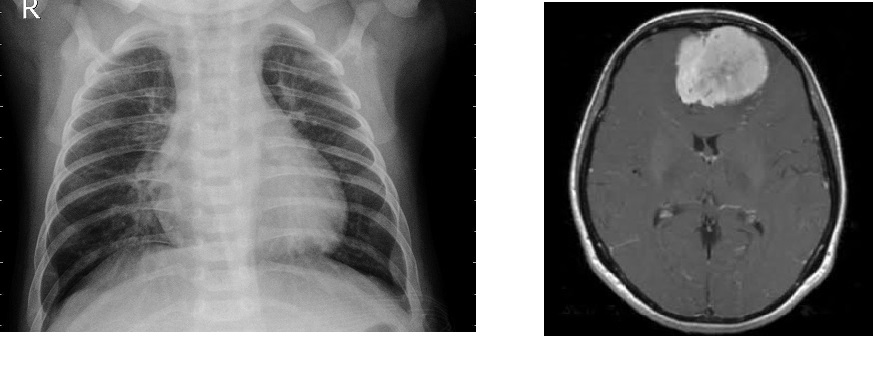
\includegraphics[width=.95\linewidth]{virus}
  %\caption{1b}
  \caption{}
  \label{fig:snap3}
\end{subfigure}
\caption{Si può notare come un soggetto sano (a) mostri polmoni senza aree di anormale opacità. L’immagine (b) è invece un caso di polmonite batterica che presenta il tipico consolidamento. (c) è un caso di polmonite virale che presenta un un'opacità interstiziale più diffusa in entrambi i polmoni.}
\label{fig:fig}
\end{figure} 

Il dataset~\cite{dspneum} è organizzato in 3 cartelle: una di Training (per l'addestramento stesso della rete), una di Testing (per testare le capacità di generalizzazione della rete) e una di Validation (per testare la bontà della rete e rilevare overfitting e/o underfitting in fase di addestramento). Ognuna di esse è organizzata così: 
\begin{itemize}
    \item 4,192 immagini per il training (1,082 casi normali, 3,110 di polmonite);
    \item 1,040 immagini di validation (267 casi normali, 773 di polmonite);
    \item 624 immagini per il testing (234 casi normali, 390 di polmonite). 
\end{itemize}
Il numero di immagini è sufficientemente grande per poter essere utilizzato per gli obiettivi preposti ricorrendo alle tecniche di deep learning per la computer vision di ambito biomedico. \\
Le proporzioni del dataset rispettano ampiamente gli standard che di solito si utilizzano per addestrare un modello di classificazione: un set di testing e uno di validation che rappresentano ognuna il 10\% del totale, il resto è lasciato al training.
Si va adesso a sintetizzare quali sono stati i principali passaggi per l’implementazione della CNN e il suo addestramento.

\subsection{Setup iniziale}
Il primo step per realizzare il classificatore è l’importazione delle librerie necessarie per la manipolazione di tensori, per le operazioni matematiche e per la relizzazione di grafici (Pandas, NumPy, MatPlotLib), così come librerie di Keras per l’image preprocessing e oggetti di Deep Learning, tra cui:
\begin{itemize}
\item \lstinline{Sequential}, classe di Keras che permette di raggruppare layers, che non sono altro che i blocchi di base per la costruzione delle reti neurali, in uno stack lineare e realizzare così un oggetto di classe \lstinline{Model}, che è implementato in modo tale da riuscire a elaborare deduzioni una volta superata la fase di training; 
\item \lstinline{Conv2D}, classe che realizza la convoluzione spaziale sulle immagini 2D. Questo strato sfrutta un kernel di convoluzione il quale è coinvolto con lo strato in input per produrre un tensore in output. Se questo strato è usato per primo nel modello è necessario inserire come parametro la tupla rappresentante le dimensioni delle immagini in input. In questo strato è possibile scegliere il numero e le dimensioni del filtro, il valore dello stride (s=1 di default), il tipo di padding e altri parametri del caso; 
\item \lstinline{MaxPool2D}, realizza l’operazione di pooling, dunque è possibile anche qui scegliere la dimensione della pool, il valore dello stride, il tipo di padding...;
\item \lstinline{Flatten}, classe che permette di trasformare la feature map allo strato precedente in un vettore che viene dato in input alla ANN in seguito;
\item \lstinline{Dense}, classe che implementa un regolare strato di una NN.
 In sostanza è questo lo strato che implementa la somma pesata degli input con i pesi e il bias 
 di cui si parlava nel capitolo 2. 
\end{itemize}

\subsection{Definizione degli iperparametri}
Successivamente sono stati fissati dei valori per gli iperparametri, ovvero quelle 
variabili poste all'inizio del codice, prima che il processo di apprendimento cominci e che possono essere modificate a piacimento fintanto che si trovano quelle che portano ai risultati migliori. 
I valori degli iperparametri sono davvero importanti per l’accuratezza del modello e delle predizioni, infatti sono stati fatti variare alcune volte prima di arrivare alla migliore soluzione. I principali sono: 
\begin{itemize}
\item Le dimensioni di input dell’immagine, perchè è necessario che durante la fase di training vi sia un'uniformità delle dimensioni degli input;
\item il numero di epoche, cioè il numero di volte in cui l’algoritmo di apprendimento 
lavora sull’intero dataset prima di procedere con l’aggiornamento dei pesi. Un'epoca descrive il numero di volte che l'algoritmo vede il intero set di dati.
Sulla base di queste varia anche la durata dell’apprendimento. Infatti gli step di apprendimento
 per epoca sono pari al rapporto tra il numero di istanze del set di training e la batch size;
\item la batch size: è un iperparametro dell’algoritmo del gradiente discendente che indica il numero di campioni di training sui quali lavorare prima che venga fatto un aggiornamento dei pesi. Sia in questa esperienza sia in quella successiva si utilizza un algoritmo di apprendimento in modalità \emph{mini-batch} in quanto il dataset è abbastanza numeroso, ovvero si utilizza un valore di batch più grande rispetto a 1, così che non si vada ad aggiornare i valori dei pesi ogni volta che il sistema riceve un campione in input, quindi più del necessario, ottimizzando la durata dell'epoca e quindi del training. Di norma la batch size deve essere un valore che sia divisore del numero totale di immagini del dataset e nelle folders. 
\item il numero di feature maps: più che ne sono più caratteristiche differenti si possono
 andare a scovare ma allo stesso tempo aumenta anche il numero di parametri e se si vuole evitare 
 il rischio di overfitting occorre aumentare la complessità del modello (ad esempio aggiungendo più strati senza perdita di troppe informazioni).
\item il numero di canali d'immagine utilizzati nel processo di learning: per le immagini RGB colorate tale parametro è pari a 3, mentre nel caso di immagini in scala di grigi vale 1. In tale caso le immagini sono digitali RGB ma vedremo che utilizzare solo un canale è la soluzione che porta ad una maggiore accuratezza in questa prima esperienza.
\end{itemize}

Facendo riferimento agli iperparametri utilizzati per la costruzione del classificatore sono stati
 scelti tali iperparametri come i migliori per questa esperienza:\\
\lstinline{img_height = img_width = 600}\\
\lstinline{epochs = 20}\\
\lstinline{batch_size = 8}\\
\lstinline{hyper_featuremaps = 32}\\
\lstinline{hyper_channels = 1}\\
\lstinline{hyper_mode = 'grayscale'}\\

E’ stata utilizzata una dimensione per le immagini di 600 x 600 pixel associata a una batch size di 8
 affinchè lo spazio occupato in RAM non sia eccessivamente alto.  \\
 Un altro iperparametro importante è il learning rate, ma il suo valore viene discusso in seguito.

\subsection{Definizione e compilazione del modello}
Per questa esperienza è stato utilizzato un modello di rete neurale convoluzionale semplice, che consiste di questi strati:\\
\begin{itemize}
\item 5 strati di Convoluzione/pooling: i primi 3 producono ognuno 32 feature maps con la convoluzione, 
generanti ognuna una feature map in seguito ad un'operazione di max-pooling. Per gli ultimi 2 sono stati invece utilizzati 64 filtri, 
così da produrre 64 feature maps anch’esse seguite da un’operazione di pooling. La convoluzione è stata performata
 con dei kernel di dimensione 3x3 e con una funzione di attivazione non lineare, cioè la ReLu. Nel capitolo precedente
  è stato indicato in parte il perchè questo tipo di funzione è quella maggiormente utilizzata in ambito di
   classificazione d’immagine. 
           L'operazione di Max-pooling viene fatta con delle pool di dimensione
           2x2. Lo stride è stato lasciato quello di default a 1 e il padding scelto è il ‘same’, affinchè la
            dimensione dell’input sia uguale alla dimensione dell’output. Viene utilizzato questo tipo di padding affinchè si abbia la certezza che il filtro venga applicato a tutti gli elementi dell'input.
\item Strato di flattening: necessario per introdurre la successiva ANN, connessa all’ultimo strato
 di pooling tramite un unico tensore unidimensionale.
\item 3 strati completamente connessi rispettivamente di 128, 64 e 1 neuroni. 
L’ultimo strato consta di un solo neurone in quanto la classificazione è binaria. 
\end{itemize}

Tipicamente si parte sempre dall’utilizzare un numero di filtri più piccolo, come in questo caso 32,
 per poi andare ad aumentare a multipli di questa dimensione. 
Il modello è infine compilato usando il metodo \lstinline{compile()} sfruttando la funzione di ottimizzazione Adam, 
algoritmo che si
 basa sull’idea del gradiente discendente ma che però elabora una stima adattativa dei momenti 
 del primo e del secondo ordine, permettendo una maggiore efficienza rispetto agli altri algoritmi
  a livello di costo computazionale per il training, a discapito di una conseguente minor capacità
   di generalizzazione. Inoltre Adam adatta il learning rate a seconda dei vari strati anche sulla base
    di quello che è il problema della scomparsa del gradiente di cui si è parlato sopra.  \\
    Con Adam il learning rate iniziale di default per il training vale 0.001 e tale valore viene poi ridotto tramite una specifica funzione quando ce ne è stato bisogno.\\
In fase di compilazione si sceglie anche la metrica, che permette di calcolare quanto spesso le label effettive
 coincidano con
 le predizioni fatte ed è dunque un parametro necessario per monitorare l’accuratezza e l’errore del modello.
  Una metrica di questo tipo viene settata col nome di \lstinline{'accuracy'}. 
  Per il calcolo dell’errore si usa una funzione di costo che in questo caso è chiamata \emph{binary crossentropy},
   (funzione di entropia incrociata binaria) poichè si va a fare una classificazione binaria.\\


   
    
\begin{python} %se voglio dividere in due pagine metto due \begin pyton separati
cnn = Sequential()
cnn.add(Conv2D(hyper_featuremaps, (3, 3), activation="relu", input_shape=(img_width, img_height, hyper_channels)))
cnn.add(MaxPooling2D(pool_size = (2, 2)))
cnn.add(Conv2D(hyper_featuremaps, (3, 3), activation="relu", input_shape=(img_width, img_height, hyper_channels)))
cnn.add(MaxPooling2D(pool_size = (2, 2)))
cnn.add(Conv2D(hyper_featuremaps, (3, 3), activation="relu", input_shape=(img_width, img_height, hyper_channels)))
cnn.add(MaxPooling2D(pool_size = (2, 2)))
cnn.add(Conv2D(hyper_featuremaps * 2, (3, 3), activation="relu", input_shape=(img_width, img_height, hyper_channels)))
cnn.add(MaxPooling2D(pool_size = (2, 2)))
cnn.add(Conv2D(hyper_featuremaps * 2, (3, 3), activation="relu", input_shape=(img_width, img_height, hyper_channels)))
cnn.add(MaxPooling2D(pool_size = (2, 2)))
cnn.add(Flatten())
cnn.add(Dense(activation = 'relu', units = 128))
cnn.add(Dense(activation = 'relu', units = 64))
cnn.add(Dense(activation = 'sigmoid', units = 1))
cnn.compile(optimizer = 'adam', loss = 'binary_crossentropy', metrics = ['accuracy'])
cnn.summary()

\end{python}
\begin{lstlisting}[caption= {Modello in Python utilizzato} ]
\end{lstlisting}

\newpage

\begin{python}
  Layer (type)                 Output Shape              Param #   
  =================================================================
  conv2d (Conv2D)              (None, 598, 598, 32)      320       
  _________________________________________________________________
  max_pooling2d (MaxPooling2D) (None, 299, 299, 32)      0         
  _________________________________________________________________
  conv2d_1 (Conv2D)            (None, 297, 297, 32)      9248      
  _________________________________________________________________
  max_pooling2d_1 (MaxPooling2 (None, 148, 148, 32)      0         
  _________________________________________________________________
  conv2d_2 (Conv2D)            (None, 146, 146, 32)      9248      
  _________________________________________________________________
  max_pooling2d_2 (MaxPooling2 (None, 73, 73, 32)        0         
  _________________________________________________________________
  conv2d_3 (Conv2D)            (None, 71, 71, 64)        18496    
  _________________________________________________________________
  max_pooling2d_3 (MaxPooling2 (None, 35, 35, 64)        0         
  _________________________________________________________________
  conv2d_4 (Conv2D)            (None, 33, 33, 64)        36928     
  _________________________________________________________________
  max_pooling2d_4 (MaxPooling2 (None, 16, 16, 64)        0         
  _________________________________________________________________
  flatten (Flatten)            (None, 16384)             0         
  _________________________________________________________________
  dense (Dense)                (None, 128)               2097280   
  _________________________________________________________________
  dense_1 (Dense)              (None, 64)                8256      
  _________________________________________________________________
  dense_2 (Dense)              (None, 1)                 65        
  =================================================================
  Total params: 2,179,841
  Trainable params: 2,179,841
  Non-trainable params: 0

\end{python}
\begin{lstlisting}[caption = {Riepilogo del modello utilizzato se in input vi è un immagine con 
  \lstinline{image_size} pari a 600. La colonna \lstinline{layer} indica il tipo di strato di cui si tratta.
   La colonna output mostra la tupla con le dimensioni dello strato in uscita (vedasi sezione 3.2.2 e 3.2.3 per
    calcolarlo), con una dimensione
    in più \lstinline{None} che è aggiunta per ospitare la batch size. La terza colonna 
    \lstinline{Param \#} indica il numero di pesi all'interno della rete, i quali possono essere
     distinti in addestrabili, cioè quelli che vengono aggiornati durante la fase di backpropagation, 
     e quelli per cui questo non vale per motivi di regolarizzazione della rete. Il numero totale di
      parametri si trova \lstinline{(kernel_height*kernel_width*input_filters+bias)* 
    output_filters}. Ad esempio nel primo strato si avra 3*3*32*1+32=320, in quanto il valore del bias è 1 di default}]
  
\end{lstlisting}

\subsection{Creazione dei set di training e validation traminte l’uso dell’image flowing}
Tramite l’utilizzo della classe di TensorFlow  \lstinline{ImageDataGenerator()} è possibile andare
 a creare dei generatori contenenti dati delle immagini di training, testing e validation in forma di tensori andando anche ad apportare modifiche ad esse. 
 
 Andando a richiamare su tali generatori il metodo  
 \lstinline{flowFromDirectory()}, è possibile ritornare un oggetto di tipo DataFrameGenerator
 costituito da una tupla (X , y) dove X è un NumPy array contenente un numero di immagini della folder indicata nel path (che vengono elaborate e rappresentate tramite i valori dei loro pixel) 
 pari alla 
   \lstinline{batch size} e della dimensione pari a  \lstinline{image_width} x \lstinline{image_height} indicata e 
   y è anch’esso
    un NumPy array che però contiene le label corrispondenti alle immagini prodotte. Proprio l'oggetto (X, y) è quello che viene dato in impasto alla rete per fare training.\\
     Durante la fase di addestramento
    viene elaborato il vettore X e per verificare se un risultato è o meno
    corretto, si compara il dato in uscita dalla rete con quello di y, dove (X, y) è la tupla ottenuta andando 
    a richiamare \lstinline{flowFromDirectory()} sul path che porta alla directory di training: se
    sono uguali allora il risultato è corretto, altrimenti il risultato necessita di
    correzioni.  L'utilizzo di
     questa funzione è stato efficace perchè il dataset è strutturato in partenza in training, 
     validation e testing. Inoltre tale funzione genera i set provvedendo a fare uno shuffle di tutte le immagini
      sia di training sia di  validation, mentre per il set di testing è stato inserito  \lstinline{Shuffle = False}
       così da poter testare la capacità di generalizzazione della rete e confrontare le predizioni con i risultati 
       effettivi, con la possibilità di scegliere a piacimento le immagini di testing su cui provare il funzionamento della rete. \\
 \lstinline{ImageDataGenarator} è una classe che permette anche di utilizzare tecniche di \emph{augmentation}~\cite{augpneum}
  per ampliare il dataset. Tali tecniche prevedono di andare a costruire versioni modificate delle immagini stesse. 
  Infatti il dataset, pur essendo numeroso, non lo è al punto tale da rendere sufficientemente buona l’esperienza
   di image processing. Questa mancanza può essere pertanto colmata andando ad ampliare il dataset con immagini
    che possano arricchire l’esperienza di training del modello. Tali immagini possono essere modificate in vari
     modi, ma non tutti questi sono utili nel caso di interesse: infatti alcune tecniche possono generare rumore 
     aggiuntivo e ''confondere'' il sistema nella ricerca dei pattern per la rilevazione della polmonite.
     Infatti è differente classificare immagini biomedicali come i raggi
     X per capire se vi è o meno una polmonite rispetto ad una classificazione di immagini come quelli di 
     cani o di gatti. Infatti, mentre un gatto può essere visto da varie angolazioni e ciò può essere
      utile al fine di distinguerlo da un cane, operare una rotazione troppo elevata per andare a riconoscere 
      l’opacità dei polmoni in un’immagine a raggi X, non va ad arricchire il dataset, ma può portare
       addirittura a un peggioramento dell’accuratezza del modello. Nell’esperienza è stato fatto un
        training del modello dapprima senza l’utilizzo di tecniche di image augmentation, per poi confrontarlo
         con un altro training in cui è stato ampliato il dataset. \\

      Occorre pertanto scegliere accuratamente quali parametri inserire. Le tecniche che sono risultate essere utili in questo caso sono:
      \begin{itemize}
        \item \textbf{Rescaling}: dato che è stata definita la modalità di colorazione 'grayscale' ogni pixel di 
        ogni immagine avrà un valore che sta nel range [0,255] che con questa tecnica diviene compreso tra 0 e 1. 
        Un primo beneficio è che così tutte le immagini vengono trattate alla stessa maniera. 
        Infatti è possibile che alcune immagini abbiano un range alto di valori dei pixel, altre più basso,
         ma entrambe condividono poi lo stesso modello e learning rate per il training. 
        In generale è bene fare in modo che il range di valori sia compreso tra 0 e 1 così che ogni immagine
         contribuisca nella maniera più uniforme possibile per il calcolo della funzione di perdita totale e 
         quindi per l'aggiornamento dei pesi. 
        \item \textbf{Rotazione}: è stato appurato che un piccolo range di rotazione per le immagini possa essere
         utile a migliorare le capacità di generalizzazione del sistema, proprio perchè molto spesso nella pratica clinica
         le radiografie possono essere lievemente ruotate a causa dei movimenti del paziente. Il range utilizzato in questo caso è tra i 
         -5$^\circ$  e i 5$^\circ$.
         \item \textbf{Zoom}: come nel caso della rotazione, è prassi che vi siano immagini in cui il torace del paziente sia posizionato
         più o meno vicino al dispositivo che elabora l'immagine. Quindi un piccolo range di variazione dello zoom delle immagini (in questo caso è stato scelto 0.2) 
         può essere utile. 
        
      \end{itemize}


      
      \begin{figure}[H]
        \centering
        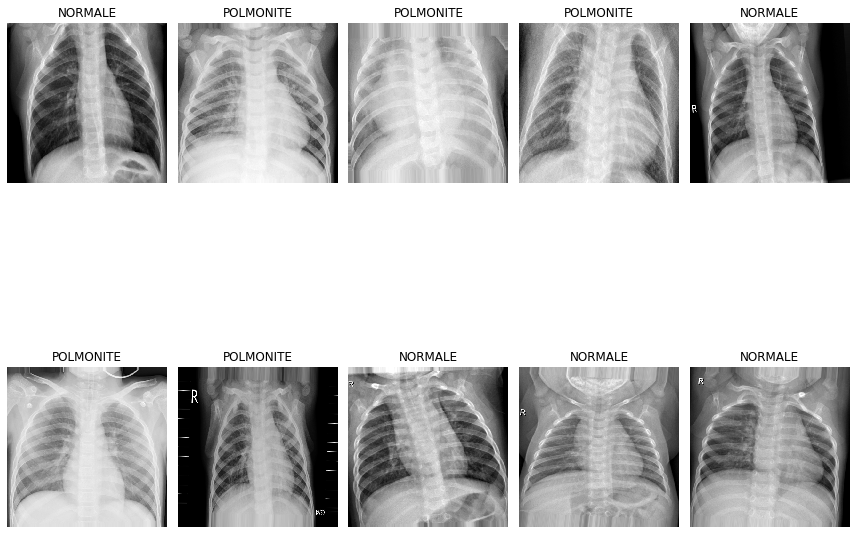
\includegraphics[width=0.9\textwidth]{Figures/best-augmented-images-pneumonia.png}
        \caption{\small{
        Campioni di immagini del dataset di training sui quali sono state aggiunte le tecniche sopra citate. Immagine tratta dal codice (vedasi capitolo 7).
        } % end small
        } % end caption
        \label{fi:dcalc}
    \end{figure}
      
     
\subsection{Fase di fitting}
Dopo aver compilato e configurato il modello si passa alla fase di \emph{fitting}, cioè la fase di addestramento
 vera e propria. Il modello viene dunque allenato tramite le immagini del set di training, con un aggiornamento
  dei pesi che viene fatto per ogni gruppo di campioni pari alla \lstinline{batchsize}. Il set di training viene rivisto
   per un totale di 20 epoche, anche se dopo 10 la capacità di training risulta essere stagnante.
    Una volta captato questo è stata usata la funzione di callback \lstinline{EarlyStopping()} che ha fermato il
     training non appena risultava esserci overfitting. 
   Il metodo  \lstinline{fit()} ci permette anche di scegliere l’insieme di validation su cui la rete 
   può generalizzare. Ciò fa sì che non solo si possa monitorare l'accuratezza nel training, ma anche la
    capacità di generalizzazione della rete, cercando di capire se questa sta andando in overfitting, 
    underfitting o se il trade-off tra le due è accettabile (Figura 5.3), così da agire di conseguenza 
    per poterla migliorare. \\
    
    \begin{figure}[H]
      \centering
      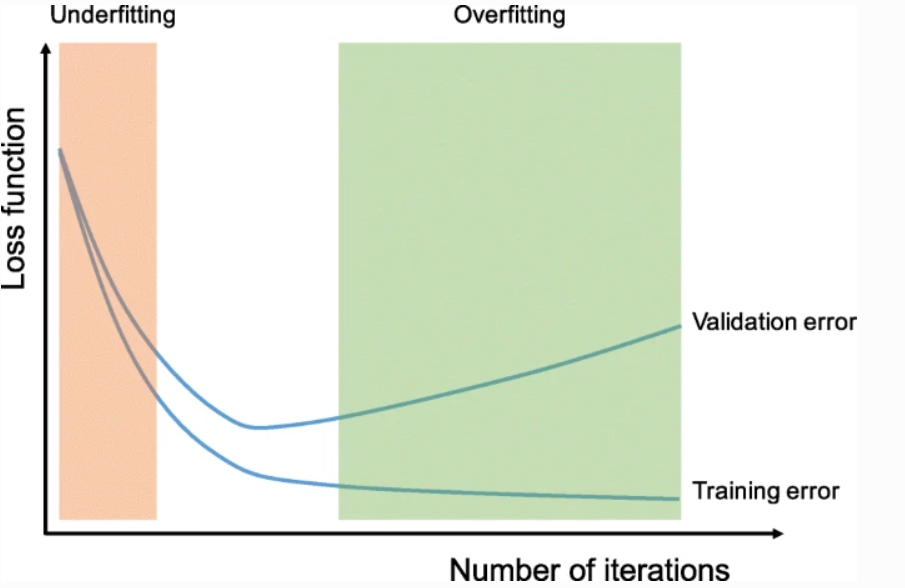
\includegraphics[width=0.9\textwidth]{Figures/ofuf (2).PNG}
      \caption{\small{Si vede come si va in overfitting quando l'errore di validation
       è molto maggiore di quello di training all'aumentare delle epoche, mentre in underfitting 
       si va quando non si hanno sufficienti parametri per allenare il modello.\cite{tesi}
      } % end small
      } % end caption
      \label{fi:dcalc}
  \end{figure}
    
    Si può anche definire una lista di chiamate (callbacks) per 
    customizzare il training, come definire un \lstinline{checkpoint} dove salvare il modello in formato \lstinline{.h5} così 
    da poterlo utilizzare successivamente per elaborare nuove predizioni,
     senza necessità di allenarlo nuovamente.  Inoltre è stata utilizzata una funzione che riduce il 
     valore del learning rate del 30\% automaticamente ogni due epoche in quanto molto spesso 
     il modello beneficia di ciò se l’apprendimento stagna. 
     %(Aprire parentesi nei capitoli precedenti di come il lr influenza l’apprendimento)
In questo caso il modello è stato allenato sull’insieme di training e validation definito dal dataset stesso.
 Il set di testing è l’insieme di immagini sulle quali si va a fare la valutazione finale.
  \begin{figure}[H]
    \begin{subfigure}{0.5\textwidth}
      \centering
      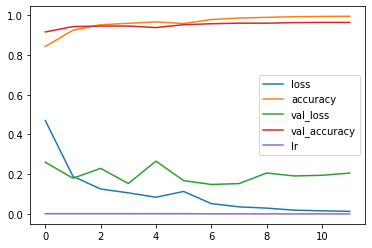
\includegraphics[width=0.95\linewidth]{Figures/history-pneumonia-no-aug.png}
      %\caption{1a}
      \caption{}
      \label{fig:snap1}
    \end{subfigure}%
    \begin{subfigure}{0.5\textwidth}
      \centering
      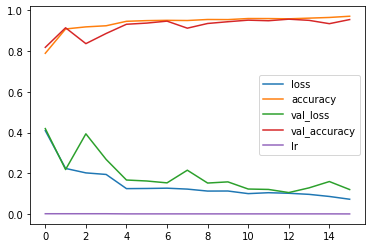
\includegraphics[width=.95\linewidth]{Figures/history-pneumonia-aug1.png}
      %\caption{1a}
      \caption{}
      \label{fig:snap2}
    \end{subfigure}%
    \caption{In entrambe le figure è possibile osservare le curve che rappresentano accuracy e 
    loss rispettivamente per training e sul set di validation nei due casi. (a) si riferisce al set 
    di training originale, (b) al set di training modificato come nella figura 5.2. Si vede che nel primo 
    caso la funzione di perdita è più alta del secondo caso. Le figure sono state create con la 
    libreria Pandas (codice capitolo 7). Il numero di epoche tra le due immagini è diverso perchè
     nel primo caso la funzione \lstinline{EarlyStopping} ha fermato il training alla undicesima epoca, nel secondo alla quindicesima.}
    \label{fig:fig}
\end{figure} 
Alla fine si ottengono questi risultati andando a richiamare \lstinline{cnn.evaluate(test)}:
\begin{itemize}
  \item Per il caso senza modifiche al set di training risulta 
  che l'accuracy sul training è pari al (99.61 $\pm$ 0.01)\% e quella
   sull'insieme di validation è del (94.44 $\pm$ 0.01)\%. Si è impiegato con l'utilizzo della CPU 
   circa 22 minuti a epoca per un totale di 20 epoche (un totale di circa 7 ore)
    per allenare il modello. Con una GPU si impiegano circa 20 secondi a epoca.
  \item  Per il caso con le modifiche al set di training risulta 
  che l'accuracy sul training è pari al (96.99 $\pm$ 0.01)\% e quella 
  sull'insieme di validation è del (94.61 $\pm$ 0.01)\%. Si è impiegato con l'utilizzo della CPU 
   circa 30 minuti per epoca per 20 epoche (un totale di circa 10 ore) per 
   allenare il modello. Con una GPU si impiegano circa 25 secondi a epoca.
  
\end{itemize}


\subsection{Predizioni e grafici}
Infine occorre osservare come il sistema riesce a generalizzare sull’insieme di test. 
Dato che la funzione di attivazione dello strato finale del modello è la sigmoide, 
il valore dell’output starà in un range compreso tra 0 e 1 corrispondente alla probabilità che l’immagine
 su cui è stata fatta la predizione presenti polmonite. 
Se si vogliono quantificare i falsi positivi e i falsi negativi occorre vedere se l’output della 
rete è superiore o inferiore a 0.5 (se è superiore o uguale risulta esserci polmonite) e di conseguenza predire se si tratta di polmonite o meno.
 É possibile visualizzare la matrice di confusione\footnote{É un modo per visualizzare in maniera 
 diretta il numero di \emph{True-positives TP} (in questo caso si intendono i soggetti che 
 sono stati previsti avere polmonite e la predizione è corretta), \emph{true-negatives TN} (il contrario),
  falsi-negativi (FN) e falsi-positivi(FP)}. 
 Le tabelle 5.1 e 5.2 rappresentano dei report di classificazione in cui è possibile osservare 3 diverse voci:
\begin{itemize}
  \item Precision = $\frac{TP}{(TP + FP)}$: rappresenta l'accuratezza di una predizione con polmonite, ma non tiene conto dei falsi negativi.
  \item Recall  = $\frac{TP}{(TP + FN)}$: rappresenta il numero di istanze con polmonite
   correttamente identificate, dunque tiene conto anche dei FN.
  \item F1 = $\frac{(2 * Precision * Recall)}{(Precision + Recall)}$: rapresenta un compromesso tra recall e precision.
  
  \item support indica il numero di immagini utilizzate come supporto al calcolo delle previsioni.\\
  \item Il valore di accuracy a cui si fa sempre riferimento è $\frac{(TP + TN)}{(TP + TN + FP + FN)}$.
\end{itemize}
Un modello deve cercare di avere il più possibile un valore di recall superiore allo 0.9 per funzionare bene.
  % Please add the following required packages to your document preamble:
% 



  \begin{table}[hb!]
  \begin{tabular}{@{}l|llll@{}}
    \toprule
                     & \textbf{precision} & \textbf{recall} & \textbf{f1-score} & \textbf{support} \\ \midrule
  \textbf{NORMALE}   & 0.93               & 0.29            & 0.44              & 234              \\
  \textbf{POLMONITE} & 0.70               & 0.99            & 0.82              & 390              \\ \midrule
  \end{tabular}
  \caption{Classification report per il modello con il set mantenuto come l'originale.}
\end{table} 
  
  

\begin{table}[H]
  \begin{tabular}{@{}l|llll@{}}
  \toprule
                     & \textbf{precision} & \textbf{recall} & \textbf{f1-score} & \textbf{support} \\ \midrule
  \textbf{NORMALE}   & 0.97               & 0.86            & 0.91              & 234              \\
  \textbf{POLMONITE} & 0.92               & 0.98            & 0.95              & 390              \\ \midrule
  \end{tabular}
  \caption{Classification report per il modello con il set ampliato.}
\end{table}

In sintesi l'accuratezza del modello sull'insieme di test vale:
\begin{itemize}
  \item  (75.80 $\pm$ 0.01)\% nella prima esperienza;
  \item  (93.75 $\pm$ 0.01)\% nella seconda.
\end{itemize}
Dunque sembra che, nonostante nella prima esperienza si abbia ottenuto un'accuratezza migliore sul training, 
poi le capacità di generalizzazione sono migliori quelle ottenute con la seconda.
 Ciò significa che nel primo training si è avuto un problema di overfitting. 


 \begin{figure}[H]
        \begin{subfigure}{0.5\textwidth}
          \centering
          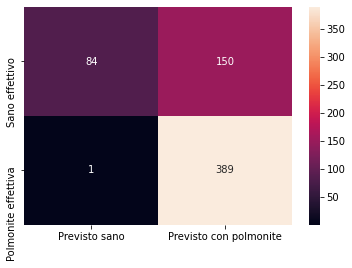
\includegraphics[width=0.95\textwidth]{Figures/conf-matrix-no-aug.png}
          %\caption{1a}
          \caption{}
          \label{fig:snap1}
        \end{subfigure}%
        \begin{subfigure}{0.5\textwidth}
          \centering
          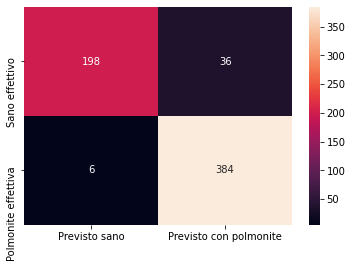
\includegraphics[width=.95\textwidth]{Figures/conf-matrix-pneumonia-aug.png}
          %\caption{1a}
          \caption{}
          \label{fig:snap2}
        \end{subfigure}%
        \caption{ Matrici di confusione ottenute. (a) è la matrice di confusione del modello con il set di
         training lasciato come l'originale. 
        Si può vedere che vi sono molti errori nel prevedere il soggetto sano. \\
        (b) è la matrice di confusione con il set di training modificato come nella Figura 5.2. 
        In questo caso vi sono pochissimi errori di predizione.
        }
        \label{fig:fig}
\end{figure} 


\begin{figure}[H]
  \centering
  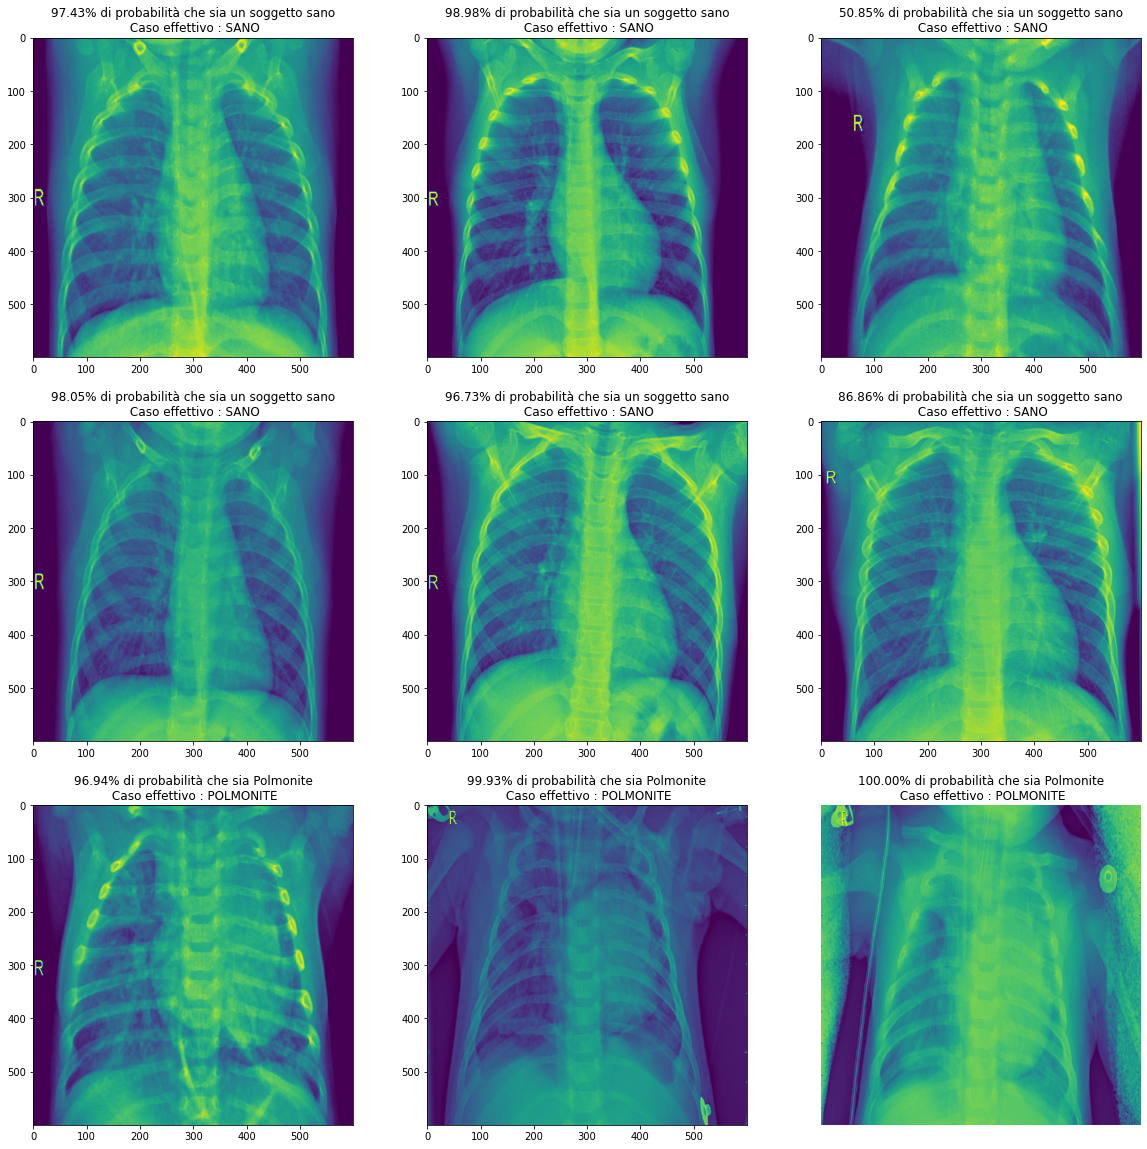
\includegraphics[width=0.9\textwidth]{Figures/pneumonia results.png}
  \caption{\small{Dimostrazione di alcune previsioni sul set della polmonite del sistema allenato con testin accuracy media del 93.75$\%$. (Codice nel capitolo 7).
  } % end small
  } % end caption
  \label{fi:dcalc}
\end{figure}
 
 
 
\subsection{Considerazioni finali}
La rete addestrata con il dataset ampliato risulta produrre buoni risultati. 
In prima istanza sicuramente grazie all’accuratezza del dataset, ma anche grazie a degli iperparametri ben scelti. In letteratura, la fase in cui si scelgono questi ultimi una volta definito il modello è chiamata \emph{fine-tuning}.
Sono state in effetti fatte delle prove con image size di dimensioni 400x400, 500x500, 600x600 e batch size = 8, 16, 32 ,
 ma la migliore accuratezza di generalizzazione si ha con gli iperparametri della sezione 5.2.3. Risultati ragionevoli 
 sono stati trovati dopo 10 epoche, anche se è stato fatto un addestramento anche con 20 e 50 epoche
 , ma ciò risultava inutile in quanto dalla decima epoca in poi l’accuratezza 
 del modello rimane costante e non migliora. Per evitare ciò è stato utilizzato l’Early Stopping che ha
  appunto fermato il modello intorno alla decima epoca. 
Inoltre è stato aumentato anche il numero dei canali d’immagine
 da 1 a 3 per osservare se vi fosse un miglioramento ma ciò non ha fatto altro che peggiorare le prestazioni. Probabilmente 
 questo è dovuto al fatto che per rilevare una polmonite la scala di grigi evidenzia maggiormente l’opacità del polmone. 
Sicuramente se il classificatore dovesse essere utilizzato in uno studio radiologico,
 sarebbe un buon mezzo di supporto in quanto il numero di falsi negativi è minore rispetto
  a quello dei falsi positivi ed è molto piccolo (clinicamente è meglio che sia diagnosticato 
  un falso positivo piuttosto che un falso negativo!). Sotto si mostrano i risultati ottenuti con iperparametri
   differenti (eccetto il numero di epoche in tutti i casi pari a 20), con le modifiche apportate al set di training della sezione 5.2.5
    e che hanno portato alla scelta di quelli alla sezione 5.2.3.

    \begin{table}[hb!]
      \begin{tabular}{l|lll}
      \hline
                                                                                                         & \multicolumn{1}{l|}{\textbf{training accuracy}} & \multicolumn{1}{l|}{\textbf{validation accuracy}} & \textbf{testing accuracy} \\ \hline
      \textbf{\begin{tabular}[c]{@{}l@{}}batch = 16\\ image size = 500x500\\ channels = 1\end{tabular}}  & 95.99\%                                         & 93.65\%                                           & 91.98\%                \\ \hline
      \textbf{\begin{tabular}[c]{@{}l@{}}batch = 32\\ image size = 400x400\\ channels = 1\end{tabular}}  & 95.94\%                                         & 95.00\%                                           & 91.5\%                 \\ \hline
      \textbf{\begin{tabular}[c]{@{}l@{}}batch = 8\\ image size = 600 x 600\\ channels = 1\end{tabular}} & 96.49\%                                         & 94.61\%                                           & 93.75\%                \\ \hline
      \textbf{\begin{tabular}[c]{@{}l@{}}batch = 8\\ image size = 600 x 600\\ channels = 3\end{tabular}} & 96.32\%                                         & 93.94\%                                           & 91.62\%                \\ \hline
      \end{tabular}
      \caption{La tabella mostra come i parametri della terza riga abbiano portato ai migliori risultati.}
      \end{table}
\newpage
\section{CNN per la classificazione di risonanze magnetiche cerebrali}
Il tumore all’encefalo è considerato una delle patologie più aggressive tra adulti 
e bambini e rappresenta circa l’85-90\% di tutti i tumori che affettano il sistema 
nervoso centrale. Ogni anno circa 11.700 persone sono diagnosticate con questo tipo 
di tumore. La percentuale di sopravvivenza per 5 anni almeno dalla diagnosi è approssimativamente del 34\% per gli uomini e del 36\% per le donne. \\ 
La miglior tecnica per rilevare il tumore all’encefalo è la risonanza magnetica (Magnetic Resonance Imaging). \\
Le RM forniscono immagini cerebrali in cui è possibile evidenziare gli effetti macroscopici
delle malattie neurologiche come ad esempio i cambiamenti di forma, intensità e dimensioni della massa tumorale. Un trattamento appropriato e una diagnostica accurata sono fondamentali per un aumento delle aspettative di vita dei pazienti. 
Un esame manuale da parte del radiologo in questo caso è ancora più complicato rispetto alla rilevazione di una polmonite e molto spesso occorre integrare tali risonanze ad altri esami aggiuntivi.
L’applicazione delle tecniche di deep learning  hanno mostrato un’accuratezza sempre maggiore anche in questo campo. Vi possono essere molte anormalità sulla grandezza e la posizione del tumore e questo rende difficile capire completamente la natura di questi. Un modello di CNN che riesca a classificare la tipologia di tumore dal semplice riconoscimento di immagine dal canto suo può essere uno strumento molto utile. É stato proprio questo l’obiettivo di realizzazione: implementare una CNN che riconoscesse tra 4 possibili stati del paziente a partire dalla semplice visione della sua risonanza magnetica. 
\subsection{Il dataset}
Il dataset~\cite{dsbrain} è stato anche in questo caso trovato nella piattaforma Kaggle e le 3264
 immagini riportano risonanze magnetiche encefaliche dove l’encefalo è visto dall’alto e
  in piano sagittale e sono raggruppate in 2 cartelle, una di Training e una di Testing.
Ognuna di esse è organizzata così: 
\begin{itemize}
\item nella training folder ci sono 395 immagini dell’encefalo sano, 827 del tumore ipofisario, 822 del meningioma e 826 del glioma. 
\item nella testing folder ci sono 105 immagini di encefalo sano, 74 di tumore ipofisario, 115 di meningioma e 100 di glioma. 
\end{itemize}
La differenza tra i diversi adenomi sta nella forma della massa tumorale e 
la posizione in cui questa si trova, proprio perchè l'origine del tumore è differente.
 Ad esempio il glioma si sviluppa nelle cellule 
della glia e può insorgere in uno qualsiasi dei due emisferi cerebrali, mentre 
il meningioma cresce quasi sempre intorno alla parete meningea ed ossea. Il tumore
 ipofisario prende origine dalla adenoipofisi e dunque è localizzato più internamente
  nell’encefalo rispetto agli altri. \\
Dunque il modello deve essere in grado di riconoscere e classificare l’immagine 
esclusivamente lavorando su queste caratteristiche.\\ 
Una classificazione di questo tipo è detta \emph{multiclasse}. 
\begin{figure}[H]
  \centering
  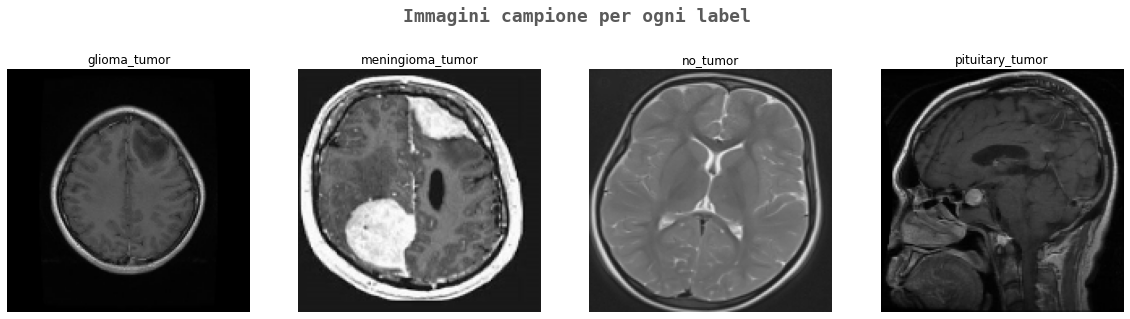
\includegraphics[width=1.1\textwidth]{Figures/brain-samples.png}
  \caption{\small{Campione di risonanza magnetica per ognuna delle diagnosi. (Disponibile codice in sezione 7)
  } % end small
  } % end caption
  \label{fi:dcalc}
\end{figure}
Non si conoscono dettagli sui pazienti ai quali è stata fatta la risonanza.
Inoltre, in questo caso il dataset è abbastanza povero per poter andare a classificare 4 
categorie di patologie differenti. Proprio per questo è stato utilizzato un modello con più strati e varie tecniche per ampliare il dataset . \\
\subsection{Setup iniziale}
 Come nell’esperienza precedentemente illustrata, anche in questo caso la prima cosa da fare 
 è importare le librerie necessarie per la creazione del modello e anche in questo caso le classi
  importate sono le stesse della sezione 5.2.2. In più però sono stati inseriti nei modelli utilizzati
  degli strati aggiuntivi, in particolare i due che seguono.
\begin{itemize} 
\item \lstinline{Dropout Layer}:~\cite{dropout} come accennato sopra, il dimensionamento di una Rete Neurale è 
un compito compless. Una Rete Neurale troppo
 piccola potrebbe non essere in grado di riconoscere abbastanza
tratti per classificare efficacemente gli ingressi, mentre una troppo grande potrebbe ottenere 
prestazioni estremamente buone in fase di addestramento ma ottenerne di pessime in fase di test,
 poichè durante l’addestramento ha sviluppato delle attivazioni nascoste che le permettevano di ottenere
  un maggior livello di accuracy sul training. É buona norma dimensionare una rete leggermente in eccesso 
  (rispetto a quanto si pensa sia ottimale o a quanto risulta ottimale) per poi utilizzare il Dropout,
   metodo per evitare la creazione delle attivazioni nascoste. 
   Lo strato di Dropout infatti fa sì che
    le unità che riceve in input un determinato strato della rete vengano randomicamente settate a 0 con una frequenza che deve essere 
    inserita come parametro. Essa indica la probabilità che un neurone si sconnetta dai suoi precedenti.
     Il Dropout fa sì che la rete impari informazioni più robuste proprio perché viene ridotto in maniera
      casuale in numero di connessioni, così che i nodi rimasti connessi dovranno regolare i propri pesi 
      per adattarsi all’assenza dei nodi non connessi, scalando i pesi di un valore tale che la somma 
      pesata degli input sia sempre la stessa. Ciò permette di ridurre overfitting, se posizionati nei punti giusti.
       Di solito uno strato di Dropout viene posizionato con un rate di 0.5 tra uno strato denso e l’altro della CNN.
       \begin{figure}[H]
        \centering
        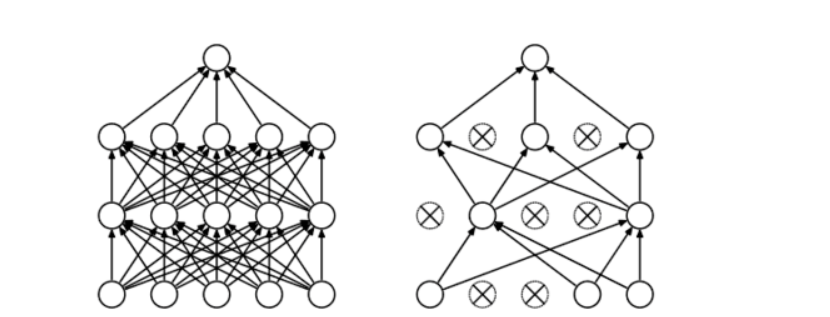
\includegraphics[width=0.8\textwidth]{Figures/dropout.png}
        \caption{\small{Dimostrazione schematica di cosa fa il dropout~\cite{dropout}. La prima immagine
         rappresenta una rete neurale connessa senza dropout, mentre la seconda rappresenta la rete dopo il dropout. .
        } % end small
        } % end caption
        \label{fi:dcalc}
      \end{figure}
\item \lstinline{BatchNormalization Layer}~\cite{norm}:  serve anche questo a dare maggior robustezza alla rete.
 Le ragioni per le quali essa funziona sono ancora sotto discussione. Si crede che questo possa mitigare il problema dello \emph{spostamento della covarianza interna}, secondo il quale l’inizializzazione di parametri e i cambiamenti nella distribuzione degli input, portano gli strati nascosti a doversi adattare ai nuovi, rallentando il training della rete. Altri studiosi pensano che invece tale strato porti al problema dell’esplosione del gradiente, contrario di quello di cui si discuteva nella sezione 3.2.3. Altri ancora negano ciò che è stato detto sopra, affermando che tale strato semplicemente serve a fare uno \emph{smoothing} della funzione di errore.  Sta di fatto che di solito se posizionati subito dopo gli strati di convoluzione in una CNN, rappresentano delle tecniche euristiche utili per il miglioramento del training.
\end{itemize}
\subsection{Definizione degli iperparametri e dei modelli utilizzati}
In questa esperienza sono stati utilizzati 3 modelli differenti e per ognuno di essi sono stati testati vari iperparametri.\\


All'inizio è stato utilizzato un modello molto simile a quello della sezione 5.2.4 
ma con più strati e filtri in quanto è stato pensato che l'estrazione di una maggior quantità di features potesse essere utile per sopperire alla grandezza limitata del dataset a disposizione.\\ 
Successivamente è stato utilizzato un modello con architettura  nota ovvero \textbf{AlexNet}~\cite{alexnet}\footnote{Il nome di questa archittura viene da Alex Krizhevsky, un computer scientist ucraino, che con tale CNN ha vinto l'ImageNet Challenge nel 2012. Il progetto ImageNet è un ampio database, nato per la ricerca software nel campo della \emph{visual object recognition}. }, la prima implementazione di una CNN basata sull'utilizzo della GPU per accelerare il training ad avere vinto un contest di riconoscimento di immagine. Vi sono diverse versioni di tale rete e quella utilizzata in tale esperienza è stata riadattata rispetto all'originale in modo da soddisfare gli obiettivi preposti per la classificazione. \\
Infine è stato utilizzato un modello pre-addestrato di una rete chiamata EfficientNetB0~\cite{effnet}\footnote{EfficientNet
 si basa sullo studio dello \emph{scaling} delle reti. Scalare una rete è qualcosa che viene fatto per 
incrementare l'accuracy di una CNN. Fare scaling di una CNN significa ridimensionare questa, e ciò può essere fatto
in profondità (andando a aumentare il numero di strati di una CNN), in larghezza (andando a regolare il numero di filtri)
 e per risoluzione (andando a mettere in input immagini più o meno rumorose). É necessario andare a bilanciare
questi 3 fattori tra loro e gli autori di questa rete hanno fatto vari esperimenti andando a utilizzare
diversi valori di scaling fino a proporre un coefficiente composto che andasse a definire 
un buon legame tra di essi, tirando fuori una nuova famiglia di modelli che hanno raggiunto un'efficienza e un'accuratezza molto alte (ad oggi 84.3$\%$ per ImageNet)} tramite una tecnica chiamata \emph{Transfer Learning}, la quale si basa sull'utilizzo di reti precedentemente allenate su un dataset differente. In effetti i primi strati di una CNN molto profonda in genere contengono estrattori di feature più generiche (esempio rilevatori di bordi o di blob di colore) mentre quelli finali sono più specifici per una singola classificazione. Pertanto andando a utilizzare i pesi inizializzati della rete preformata e andando a riqualificare gli ultimi strati a seconda del caso di interesse, è possibile che si riescano ad estrarre le feature anche dai nuovi dati. 

Sotto si riportano dunque le architetture dei 3 modelli utilizzati:
\begin{enumerate}
    \item Una CNN generica con 4 strati di convoluzione 2D (sono stati utilizzati 32, 32, 64 e 128 filtri per strato) ognuno seguito da una BatchNormalization,
     disposti in due blocchi alla fine dei quali sono stati aggiunti due strati di MaxPooling-Dropout. \\
    I Fully Connected Layers sono 3, uno con 512, l'altro con 128 e l'ultimo con 4, 
    ognuno intervallato da una BatchNormalization. \\
    Le funzioni di attivazione sono sempre ReLu per tutti gli strati nascosti e l'ottimizzatore 
    scelto è Adam (sarà così anche per i modelli successivi) in quanto risultano essere i migliori per quanto riguarda un buon compromesso tra durata del training e accuratezza della rete. \\
    
    La funzione di perdita utilizzata nella classificazione multipla è
     la \lstinline{categorical_crossentropy}, la quale permette la realizzazione
      dell'algoritmo di backpropagation calcolando l'errore di previsione tra il 
      vettore rappresentante la label di target (infatti in questo caso la coppia 
      immagine-label presenta un numero di label codificato in codice 
      one-hot\footnote{tipo di codifica in cui viene rappresentato un numero intero positivo attraverso un vettore che contiene solamente zeri eccetto la cella puntata dall’indice corrispondente all’intero positivo che si vuole codificare.}) e il vettore di stima elaborato fino a quel momento.
  Per i vari training eseguiti sono stati utilizzati questi iperparametri:
  \begin{itemize}
    \item 
  
  Una \lstinline{image_size = 150} dove si intende che tutte le immagini in input alla rete
   sono state, una volta lette, ridimensionate con un numero di pixel pari a \lstinline{image_size} x \lstinline{image_size}. \\
  A questa è stata associato un valore di \lstinline{batch_size} che è stato fatto variare tra 
  8, 32 e 64. Successivamente è stata utilizzata anche una \lstinline{image_size} di 224; 
 \item Il numero di epoche è stato posto inizialmente per tutti i modelli pari a 40 ma poi il numero è stato ridotto in quanto si è notato che il training risultava essere stagnante su un minimo già molto prima della 40-esima epoca; 
\item Il valore di \lstinline{hyper_featuremaps} è stato posto pari a 32 e mano a mano che si giunge più in profondità il numero dei filtri raddoppia (64 filtri nel terzo strato) e 
quadruplica (128 filtri nel quarto), come è possibile vedere nel code listing sotto;
\item \lstinline{hyper_channels = 3}, ma è stato tentato un training anche con tale valore pari a 1. \\

\end{itemize}
\newpage

    \begin{python}
model = Sequential()
model.add(Conv2D(hyper_featuremaps, kernel_size=(3, 3), activation='relu', input_shape=(image_size,image_size, hyper_channels)))
model.add(BatchNormalization())

model.add(Conv2D(hyper_featuremaps , kernel_size=(3, 3), activation='relu'))
model.add(BatchNormalization())
model.add(MaxPooling2D(pool_size=(2, 2)))
model.add(Dropout(0.25))

model.add(Conv2D(hyper_featuremaps*2, kernel_size=(3, 3), activation='relu'))
model.add(BatchNormalization())
model.add(Dropout(0.25))

model.add(Conv2D(hyper_featuremaps*4, kernel_size=(3, 3), activation='relu'))
model.add(BatchNormalization())
model.add(MaxPooling2D(pool_size=(2, 2)))
model.add(Dropout(0.25))

model.add(Flatten())

model.add(Dense(512, activation='relu'))
model.add(BatchNormalization())

model.add(Dense(128, activation='relu'))
model.add(BatchNormalization())
model.add(Dense(4, activation='softmax'))

model.compile(loss=keras.losses.categorical_crossentropy,
              optimizer=keras.optimizers.Adam(),
              metrics=['accuracy'])
    \end{python}
    \begin{lstlisting}[caption= {Codice Python del primo modello utilizzato.} ]
    \end{lstlisting}
    \item AlexNet ~\cite{alexnet}s nella sua prima versione del 2012 era costituito da 8 strati di cui 5 di convoluzione e 3 fully-connected da 4096,
     4096 e 1000 unità in quanto tale rete è nata per una classificazione per 1000 classi diverse. AlexNet è nato infatti per un dataset di larga scala come ImageNet, 
     con più di 15 milioni di immagini ad alta risoluzione appartenenenti a più di 22.000 categorie differenti. Per mantenere l'architettura il più simile possibile 
     a quella originale tutti gli strati sono stati mantenuti, ma ne è stato aggiunto un nono per andare a classificare le 4 tipologie di diagnosi, dunque di 4 unità.
     Il primo strato di convoluzione filtra un'immagine con \lstinline{image_size=150} e \lstinline{hyper_channels = 3} con uno stride di 4 pixel. 
     Il secondo strato convoluzionale prende in input l'output (normalizzato e passato per la pool) del primo strato di convoluzione con 256 filtri di dimensione 5×5.
      Da qui in poi lo stride per la convoluzione è sempre pari ad 1, mentre è pari a 2 quello per il pooling. \\
     Il terzo, il quarto e il quinto strato di convoluzione sono connessi tra loro  senza essere separati da uno strato di pooling. 
     Il terzo strato di convoluzione ha 384 kernel di dimensione 3x3 e così il quarto, mentre il 
     quinto utilizza 256 filtri ed è seguito da uno strato di Max-Pooling.\\
     É stata scelta questa rete perchè non troppo complessa tra le reti più conosciute e facile da manipolare e riutilizzare
      anche per altri tipi di classificazione.
      \begin{figure}[hb!]
        \centering
        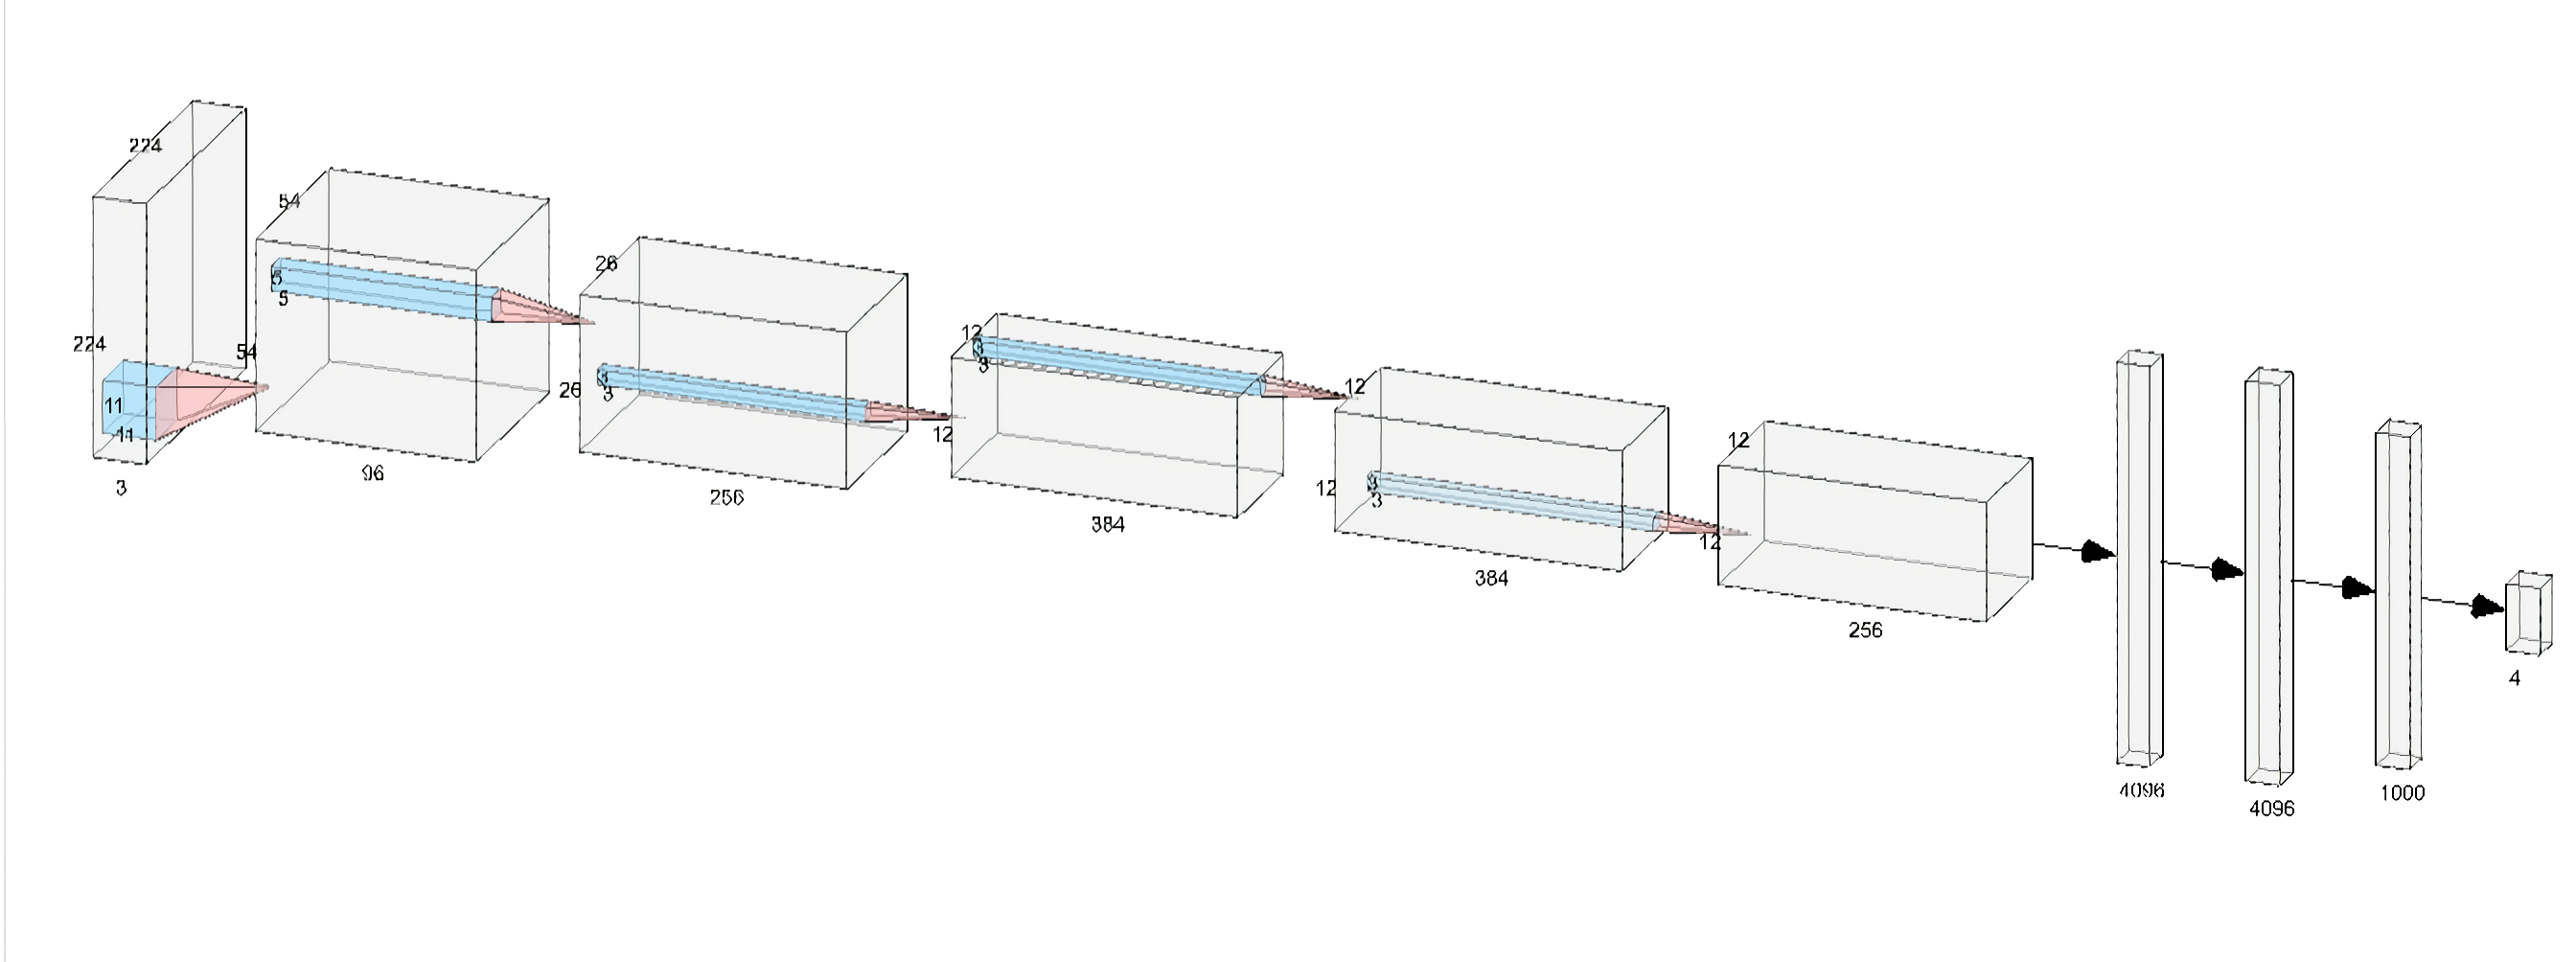
\includegraphics[width=0.9\textwidth]{Figures/alexnet.png}
        \caption{\small{schema di Alexnet riadattato, realizzato con NNSVG.} % end small
        } % end caption
        \label{fi:dcalc}
      \end{figure}
      \\
\newpage
\begin{python}
model = keras.models.Sequential([
keras.layers.Conv2D(filters=96, kernel_size=(11,11), strides=(4,4), activation='relu', input_shape=(image_size,image_size,3)),
keras.layers.BatchNormalization(),
keras.layers.MaxPool2D(pool_size=(3,3), strides=(2,2)),
keras.layers.Conv2D(filters=256, kernel_size=(5,5), strides=(1,1), activation='relu', padding="same"),
keras.layers.BatchNormalization(),
keras.layers.MaxPool2D(pool_size=(3,3), strides=(2,2)),
keras.layers.Conv2D(filters=384, kernel_size=(3,3), strides=(1,1), activation='relu', padding="same"),
keras.layers.BatchNormalization(),
keras.layers.Conv2D(filters=384, kernel_size=(3,3), strides=(1,1), activation='relu', padding="same"),
keras.layers.BatchNormalization(),
keras.layers.Conv2D(filters=256, kernel_size=(3,3), strides=(1,1), activation='relu', padding="same"),
keras.layers.BatchNormalization(),
keras.layers.MaxPool2D(pool_size=(3,3), strides=(2,2)),
keras.layers.Flatten(),
keras.layers.Dense(4096, activation='relu'),
keras.layers.Dropout(0.5),
keras.layers.Dense(4096, activation='relu'),
keras.layers.Dropout(0.5),
keras.layers.Dense(1000, activation='relu'),
keras.layers.Dropout(0.5),
keras.layers.Dense(4, activation='softmax')])
model.compile(loss=keras.losses.categorical_crossentropy, optimizer=keras.optimizers.Adam(), metrics=['accuracy'])
    \end{python}
    \begin{lstlisting}[caption= {Codice Python del modello di AlexNet riadattato.} ]
    \end{lstlisting}

    \item Nella terza fase di questa esperienza si applica il concetto di Transfer Learning.
     Viene infatti utilizzato un modello già allenato per il dataset ImageNet, ovvero \lstinline{EfficientNetB0}. 
    La funzione omonima \lstinline{EfficientNetB0()} ritorna un modello di Keras di questo tipo. \\
    \begin{figure}[H]
      \centering
      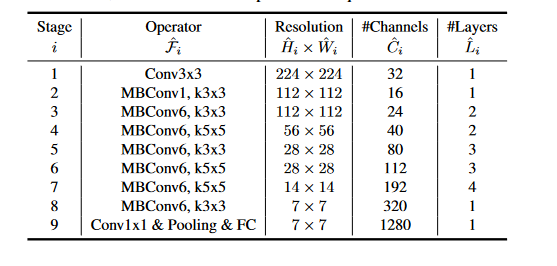
\includegraphics[width=0.8\textwidth]{Figures/EfficientNet.png}
      \caption{\small{Immagine presa dal paper di EfficientNet. Essa mostra come è fatta l'architettura di EfficientNetB0. Ogni riga descrive un passaggio i con un numero 
      \emph{$L_i$} di strati, con risoluzione in input pari a $H_i$ x $W_i$ e numero di filtri in output pari a $C_i$.
      Si sfrutta uno strato di convoluzione seguito da 7 blocchi di MBConv (vedasi sotto) 
       e che termina con uno strato FC.
      } % end small
      } % end caption
      \label{fi:dcalc}
    \end{figure}
    
    
    Un blocco \emph{MBConv} Consiste usa un approccio \emph{narrow-wide-narrow}~\cite{mobilenet} con una convoluzione 2D 1x1 seguita da una
    convoluzione depthwise che permette di ridurre il costo computazionale del training e che riduce il
     numero di parametri. Dopo di che, un altro strato di convoluzione fa uno squeezing della rete così che il numero
     di filtri coincida con quello desiderato.\\
     Con la convoluzione Depthwise si può vedere come effettivamente da 80 milioni di paramentri si passa a solo 4 milioni circa se gli iperparametri sono quelli isceriti nei code listings sopra. 
    \begin{python}
  def MCConv1(x, expand=expansion_number, squeeze=squeeze_number):
  m = Conv2D(expand, (1,1))(x)
  m = BatchNormalization()(m)
  m = Activation('relu6')(m)
  m = DepthwiseConv2D((3,3))(m)
\end{python}

\begin{python}
  m = BatchNormalization()(m)
  m = Activation('relu6')(m)
  m = Conv2D(squeeze, (1,1))(m)
  m = BatchNormalization()(m)
  return Add()([m, x])
  \end{python}
   La funzione EfficientNetB0 di TensorFlow dà la possibilità di settare il parametro \lstinline{include_top = False}, così che gli strati 
    densi del modello originale non vengano importati in modo da riadattare la sua architettura agli obiettivi di questo lavoro.\\
    In effetti gli strati densi del modello e l'operazione di \lstinline{Flattening} sono stati successivamente sostituiti
     dall'operazione di \lstinline{GlobalAveragePooling2D}, equivalente al MaxPooling
    ma che utilizza il valore medio per ogni feature map anzichè il massimo 
    e che utilizza una pool di dimensione pari alle dimensioni delle mappe di input. Successivamente, si aggiunge
     un Dropout e infine uno strato denso che consenta la classificazione delle 4 categorie.  
    
    \begin{python}
effnet = EfficientNetB0(weights='imagenet',include_top=False,input_shape=(image_size,image_size,hyper_channels))
model = effnet.output
model = tf.keras.layers.GlobalAveragePooling2D()(model)
model = tf.keras.layers.Dropout(rate=0.5)(model)
model = tf.keras.layers.Dense(4,activation='softmax')(model)
model = tf.keras.models.Model(inputs=effnet.input, outputs = model)
model.summary()   
model.compile(loss='categorical_crossentropy',optimizer = 'Adam', metrics= ['accuracy'])
\end{python}
\begin{lstlisting}[caption= {Codice realizzato per applicare il Trasfer Learning.} ]
\end{lstlisting}

    
    I 3 modelli hanno in comune lo stesso ottimizzatore cioè Adam e la stessa funzione di perdita, 
    così come le funzioni di attivazione 
    utilizzate (eccetto EfficientNet che utilizza talvolta la \emph{swish} al posto della ReLu), in modo
     particolare quella dell'ultimo 
    stato che è la \emph{softmax}. Questa è infatti utilizzata 
    di prassi nella classificazione multipla. Essa comprime un vettore \emph{z} k-dimensionale a
     valori reali in un vettore 
    k-dimensionale $\sigma(z)$ di valori compresi nell'intervallo (0,1) la cui somma è 1.\\
    Applicare la softmax significa prendere in considerazione tutti gli elementi dell'output dell'ultimo
     strato e definire da questi una funzione di probabilità considerandoli correlati tra loro.
     In effetti la funzione è di questo tipo: \[softmax(z_j) = \frac{\mathrm{e}^{z_j}}{\sum_{k=1}^{K}\mathrm{e}^{z_k}} \]
     dove K è il numero di classi. Dunque nel caso di interesse in output alla rete di otterrà un vettore 4x1 ove ogni riga k
      rappresenta la distribuzione di probabilità per cui l'input dato in impasto alla rete possa appartenere
       alla k-esima classe. Ovviamente tale funzione è strettamente legata all'uso della funzione
        di entropia incrociata categorica.
    
  \end{enumerate}

\subsection{Creazione dei set di training e testing}
Dopo aver letto (utilizzando la libreria \lstinline{openCV}) e ridimensionato tutte le immagini,
 queste vengono inserite in un array \textbf{X} il quale
 viene convertito poi in un NumPy array in cui ogni elemento è associato all'array di label \textbf{y} corrispondenti tra le 4 possibili, 
  come prevede  l'apprendimento supervisionato.\\ \\
 \lstinline{labels = ['glioma_tumor','meningioma_tumor','no_tumor','pituitary_tumor']} \\
 
  Questa volta per questo tipo di dataset è stato deciso di utilizzare la funzione  della libreria \lstinline{scikit}
 ovvero \lstinline{train_test_split}, che permette di suddividere la coppia (X, y) in due set di training e testing,
  dando la possibilità di decidere le dimensioni dei due rispetto al totale degli elementi
   e di fare uno shuffle a questi,
  così che l'apprendimento sia più robusto (ovviamente ogni volta che si richiama tale funzione si ottengono 
  set di testing e training diversi,
   pertanto i risultati ottenuti possono variare leggermente gli uni dagli altri) É stato scelto un set di
    testing pari al 10\% del totale, dunque 327 elementi 
  contro i 2894 del training, poichè si è preferito lasciare il massimo numero di immagini possibili
   riservate all'apprendimento.
  Ovviamente a seconda di come vengono disposte le immagini nel set di training e in quello di testing si possono 
  ottenere risultati differenti per quanto riguarda l'accuratezza della rete, pertanto in media sono
   stati fatti 5 training per ogni modello.
   In questo caso non avendo a disposizione
   un dataset sufficientemente fornito, cosa abbastanza tipica dei dataset biomedicali, è stato deciso 
   di far coincidere set di validazione e set di testing. 
  A questo punto si è operato in maniera differente per ognuno dei 3 modelli 
  descritti alla sezione precedente. 
\subsection{Fase di fitting e predizioni}
  \begin{enumerate}
    \item Con il primo modello il numero di parametri da allenare è piuttosto alto (75,932,388 parametri se l'immagine di ingresso ha 
    \lstinline{image_size = 150})
    causa il grande numero di filtri applicati e di unità negli strati densi. 
    Inizialmente è stato fatto un aumento del numero di immagini con tecniche simili a quelle applicate
     nel dataset precedente
    ma ciò non ha portato a
     miglioramenti rispetto all'accuratezza sull'insieme di test.\\
     Questo perchè in questo caso ciò che comporta una maggiore accuratezza alla rete 
     è la capacità di distinguere la forma di un un meningioma da quella di un glioma e un adenoma
      ipofisario anche in rapporto alla posizione in cui si trovano all'interno dell'encefalo. 
      Un modello che possiede molti parametri da allenare  con l'aggiunta di immagini
      ruotate e alterate geometricamente ha portato infatti ad un lieve overfitting, 
       passando da un'accuratezza sul testing media di 92.2$\%$ (valore medio calcolato su 5 diversi training)
        a una media del 91$\%$. 
       
       Dunque si è preferito allenare questo primo modello con il set autentico e 
       ciò ha portato a risultati abbastanza soddifacenti. 
       I parametri che hanno portato ad un'accuratezza sull'insieme di test del 91.98$\%$ sono questi:\\
       \lstinline{image_size = 150} e \lstinline{batch_size = 32}; un aumento ulteriore
        della grandezza dell'immagine portava ad overfitting. \\
       \lstinline{epochs=40}, di cui in media ne sono necessarie solo 20, ognuna delle quali con la GPU aveva la durata di circa 6 secondi, 
       a fronte dei 3 minuti e 30 secondi a epoca con la necessità di almeno 20 epoche se si utilizza la CPU.\\
       \lstinline{hyper_channels = 3}, ovvero è stata mantenuta la modalità rgb con cui la libreria OpenCV legge le immagini.
       É stata fatta una prova anche con 1 solo canale ma non si sono ottenuti cambiamenti sostanziali. 
       \begin{figure}[H]
        \begin{subfigure}{0.5\textwidth}
          \centering
          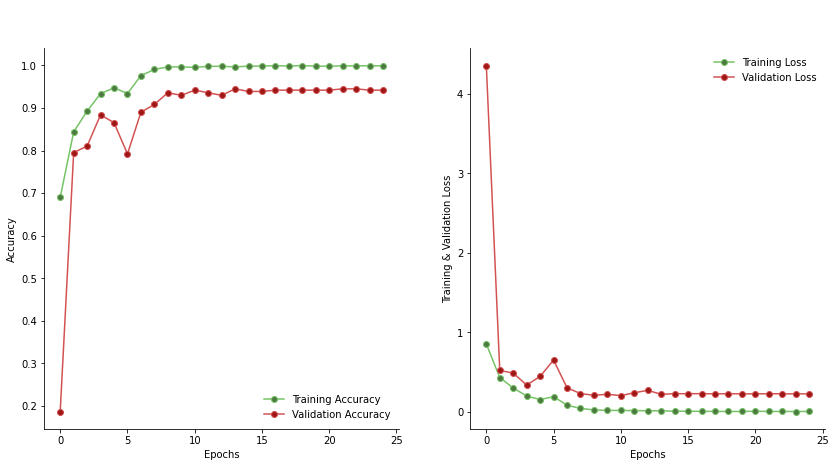
\includegraphics[width=0.95\textwidth]{Figures/history-first-model-original}
          %\caption{1a}
          \caption{}
          \label{fig:snap1}
        \end{subfigure}%
        \begin{subfigure}{0.5\textwidth}
          \centering
          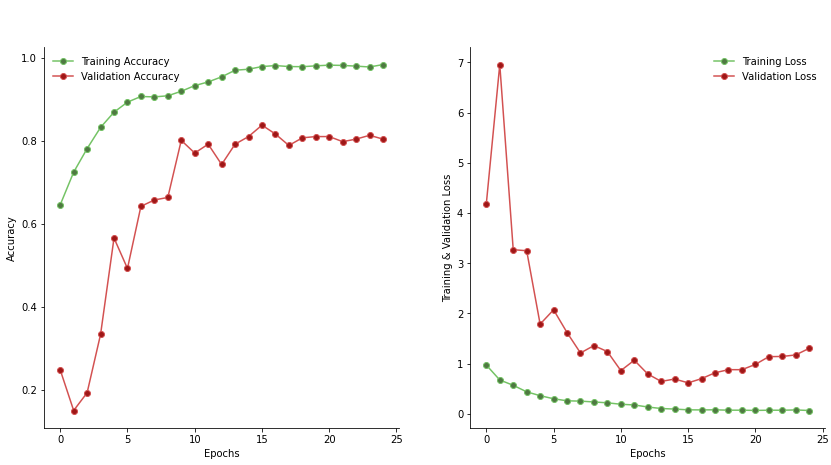
\includegraphics[width=.95\textwidth]{Figures/history-first-model-aug}
          %\caption{1a}
          \caption{}
          \label{fig:snap2}
        \end{subfigure}%
        \caption{Esempi di andamento della validation e training accuracy-loss nel training del modello 1. A sinistra il training fatto sul set originale, a destra quello fatto sul set alterato 
        Come si vede nella figura (b) il set alterato non comporta miglioramenti in fase di testing e con le epoche cresce anche l'errore di stima.}
        \label{fig:fig}
\end{figure} 

       
      
    \item Con la versione di AlexNet riadattata al caso di interesse i risultati ottenuti senza ampliare il dataset
    sono stati un'accuratezza sul training del 98$\%$ e sul testing del (92.6 $\pm$ 1)$\%$. 
    Anche in questo caso, come per il modello precedente, andare a ad applicare tecniche di ampliamento del dataset
    che alterassero la geometria delle immagini non è stato molto utile e così nemmeno andare a traslare o ingrandire l'immagine, 
    questo perchè la caratteristica principale delle CNN è di assicurare l'estrazione di feature che siano invarianti 
    rispetto alle traslazioni dell'immagine. \\ 
    Invece tutte quelle tecniche che non alterano geometricamente la forma dell'immagine ma solamente l'intensità dei pixel,
    sia localmente sia in tutta l'immagine, possono aiutare sicuramente nel riconoscimento di determinate forme. 
    Infatti le immagini biomedicali, in particolare quelle di questa tipologia, essendo acquisite con diversi 
    scanner e in differenti locazioni, possono essere intrinsecamente molto eterogenee nell'intensità dei pixel,
     e nella saturazione. 
    Quindi vi possono essere immagini più o meno definite e andare a regolare l'intensità dei pixel
     per tutte le immagini garantendo una 
    maggiore omogeneità tra queste è sicuramente la via migliore per incrementare
     l'accuratezza della rete~\cite{gaussnoise}.\\
    In particolare è stata applicata una perturbazione data da \emph{rumore Gaussiano}
    (di valor medio nullo) al set di
     immagini per il training, facendo variare il valore della
    deviazione standard  e accostando l'aggiunta di tale rumore ad un rescaling. Risultati buoni sono stati ottenuti con varianza pari a 2. \\
    Qui sotto dei campioni di immagini ottenute sommando al Numpy array \lstinline{X_test} ottenuto dal set di training
    originale il valore
    \begin{python}
    gaussian = np.random.normal(mean, std, (image_size, image_size,hyper_channels))
    \end{python}
    dove \lstinline{mean} è il valore medio e \lstinline{std} la varianza del segnale gaussiano generante il rumore.\\
    \begin{figure}[H]
      \begin{subfigure}{0.5\textwidth}
        \centering
        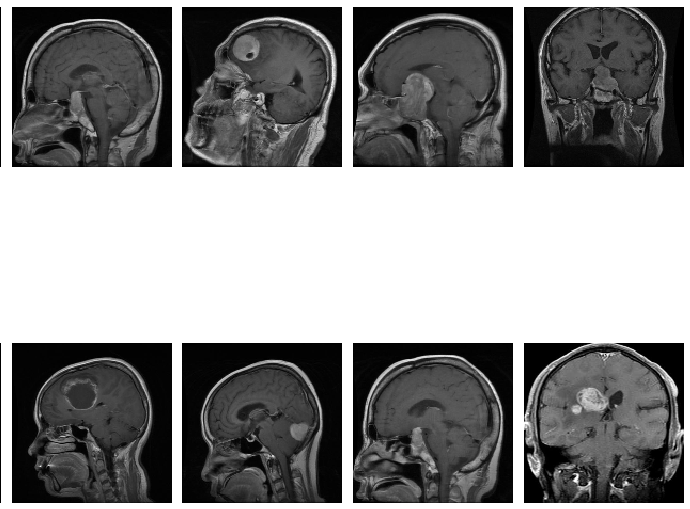
\includegraphics[width=.95\textwidth]{Figures/images-no-noise.png}
        %\caption{1a}
        \caption{}
        \label{fig:snap1}
      \end{subfigure}%
      \begin{subfigure}{0.5\textwidth}
        \centering
        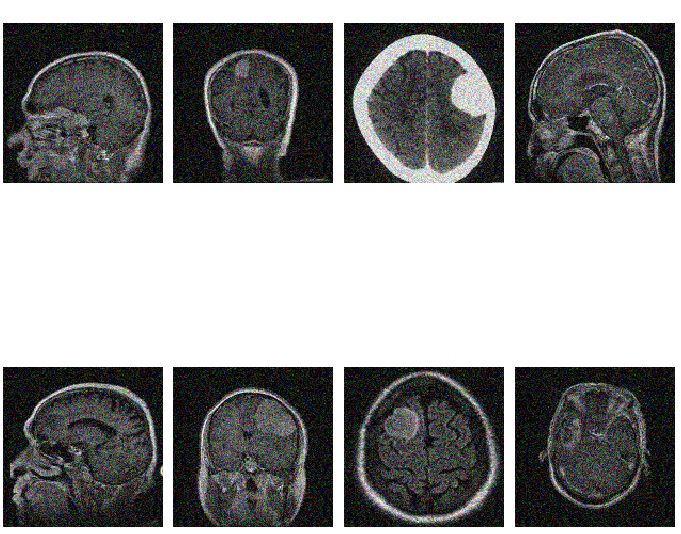
\includegraphics[width=.95\textwidth]{Figures/images-noise-var-20}
        %\caption{1a}
        \caption{}
        \label{fig:snap2}
      \end{subfigure}%
      \caption{Esempi di RM prima di aver applicato il rumore gaussiano (a) e dopo (b). In questo caso la varianza è stata posta pari a 20 volutamente esagerando per dare maggior idea di che cosa comporta, ma 
      in generale si utilizza un valore più basso per non alterare troppo le immagini.}
      \label{fig:fig}
\end{figure} 
    Successivamente è stato applicato anche un \lstinline{rescaling = 1./255} tramite \lstinline{ImageDataGenerator}.
    In questo modo è stata raggiunta un'accuratezza sul set di testing pari al (95.7 $\pm$ 1)$\%$, circa il (2-3)$\%$ in più
     rispetto al caso senza noising.
    Molti studi hanno notato infatti che aggiungere piccole quantità 
    di rumore (\emph{jitter}) nel set di training aiuta nella generalizzazione
    e per la \emph{fault tolerance}, cioè la capacità che ha la rete di continuare ad essere affidabile anche se alcune
    delle sue unità nascoste smettono di funzionare. Aggiungere rumore alle immagini significa che la rete è meno
    capace di memorizzare i campioni di training perchè questi cambiano continuamente così come le feature estratte,
    ottenendo valori dei pesi tra i neuroni più piccoli ma una maggior robustezza. Infatti se una rete viene allenata
     con immagini 
     affette da rumore sufficientemente piccolo, poi avrà maggior capacità di riconoscere i pattern nelle
      immagini di testing non affette da tale errore.
    In questo caso l'accuratezza nel training è circa del (97.5 $\pm$ 1)$\%$, quindi inferiore a quella del modello in cui non 
    è stato aggiunto il rumore, ma a discapito di una migliore performance in fase di testing. Inoltre è stato
     approvato che a parità di epoche
    il training con il rumore aggiunto raggiunge risultati migliori a livello di validation accuracy, dunque il sistema riesce ad allenarsi più velocemente. \\
    Gli iperparametri scelti sono gli stessi del modello precedente.
    \begin{figure}[hb!]
      \begin{subfigure}{0.5\textwidth}
        \centering
        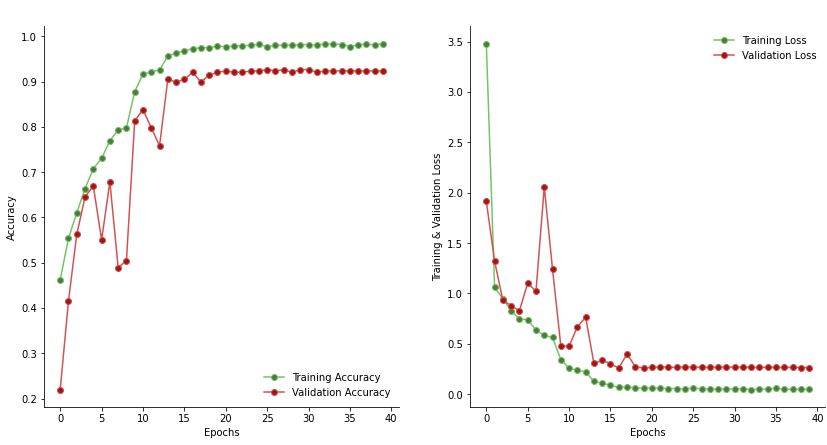
\includegraphics[width=0.95\textwidth]{Figures/history-alexnet-original.png}
        %\caption{1a}
        \caption{}
        \label{fig:snap1}
      \end{subfigure}%
      \begin{subfigure}{0.5\textwidth}
        \centering
        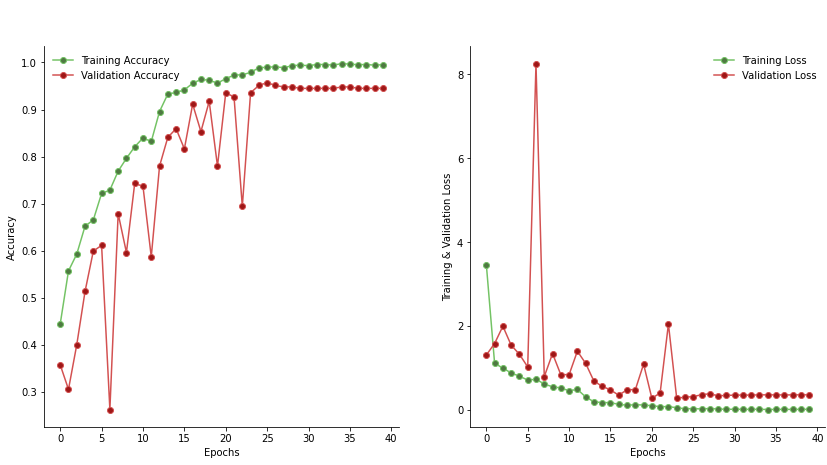
\includegraphics[width=.95\textwidth]{Figures/history-alexnet-noise.png}
        %\caption{1a}
        \caption{}
        \label{fig:snap2}
      \end{subfigure}%
      \caption{Esempi di andamento della validation e training accuracy-loss del secondo modello. A sinistra il training fatto sul set originale, a destra quello fatto sul set alterato con il rumore gaussiano. 
      }
      \label{fig:fig}
\end{figure} 

\newpage
    \item Dato che i modelli precedenti, così detti \emph{"from scratch"}, hanno
     raggiunto risultati non superiori al (95.7 $\pm$ 1)$\%$, è stato 
    eseguito il training sul modello di EfficientNet descritto al punto 3 della sezione precedente.
     In questo caso in 14 epoche 
    è stata raggiunta un'accuratezza sia sul training sia sul testing in media del (99 $\pm$ 0.1)$\%$.
    Infatti per le tecniche sopracitate di tipo depth-wise utilizzate nell'architettura del modello il numero di parametri,
     sempre con \lstinline{image_size = 150}, \lstinline{batch_size = 32} e \lstinline{hyper_channels=3} si ottengono solo 4,054,695 parametri,
      di cui circa 42 000 di tipo non-trainable.\\
    
     In dataset piccoli come questo infatti il concetto di transfer-learning
    basato su modelli allenati sull'ImageNet rappresenta lo stato dell'arte per 
    i problemi di classificazione e segmentazione di immagine.
  \end{enumerate}
    \begin{figure}[hb!]
      \centering
      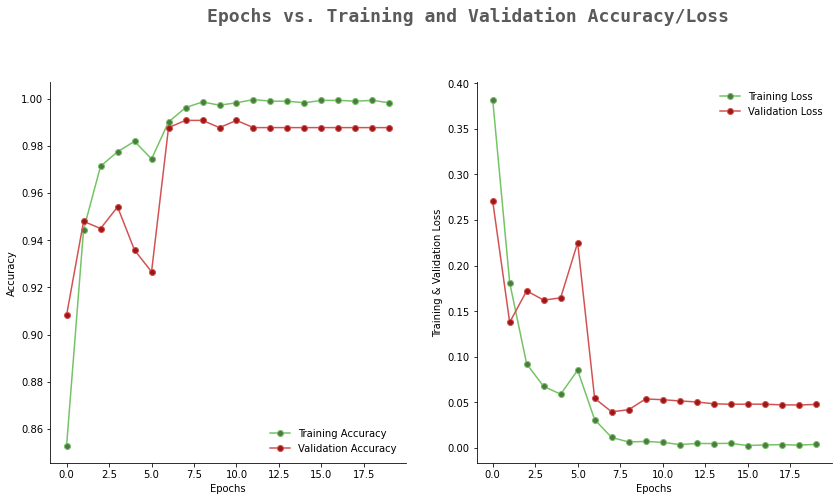
\includegraphics[width=0.8\textwidth]{Figures/history-model-pretrained.png}
      \caption{\small{Andamento della training-validation accuracy e loss del modello 3.} % end small
      } % end caption
      \label{fi:dcalc}
    \end{figure}
    Si riportano le tabelle riferite alla capacità di predizione della rete in seguito 
    all'utilizzo dei 3 modelli e le matrici di 
    confusione corrispondenti.
    \begin{figure}[H]
      \begin{subfigure}{1\textwidth}
        \centering
        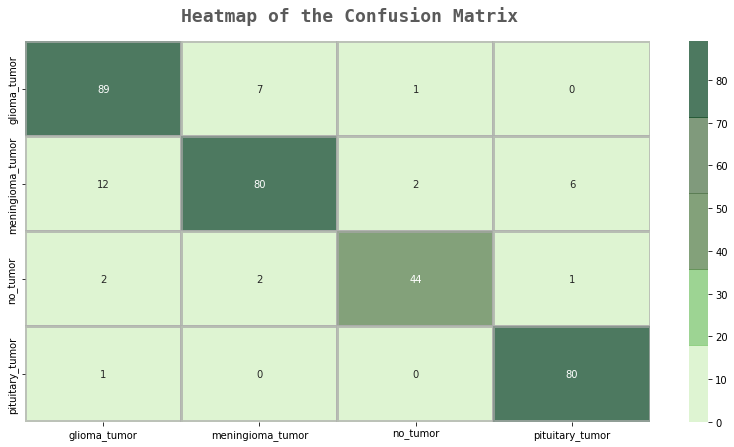
\includegraphics[width=0.60\linewidth]{conf-matrix-first.png}
        %\caption{1a}
        \caption{}
        \label{fig:snap1}
      \end{subfigure}\\
      \begin{subfigure}{1\textwidth}
        \centering
        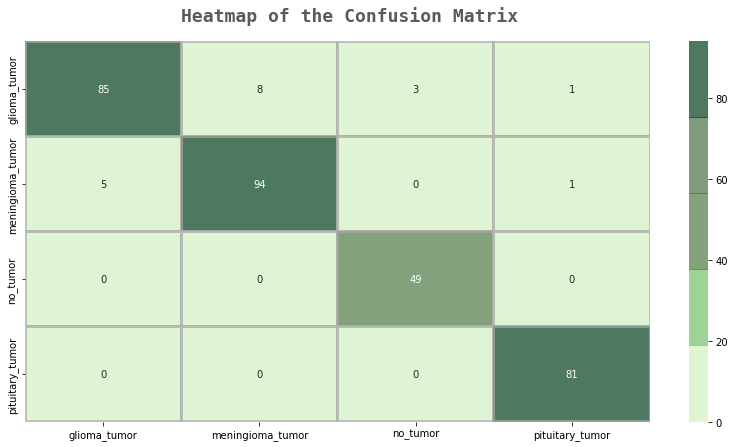
\includegraphics[width=0.60\linewidth]{conf-matrix-alex.png}
        %\caption{1a}
        \caption{}
        \label{fig:snap2}
      \end{subfigure}\\
      \begin{subfigure}{0.93\textwidth}
        \centering
        
        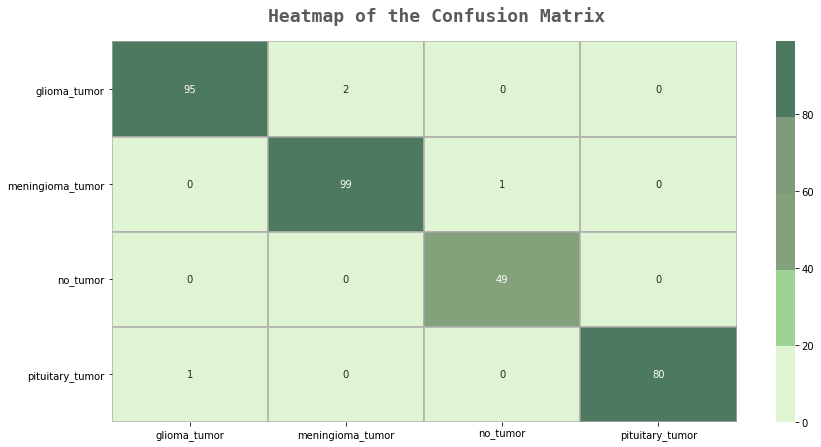
\includegraphics[width=0.75\linewidth]{conf-matrix-pretrained.png}
        %\caption{1b}
        \caption{}
        \label{fig:snap3}
      \end{subfigure}
      \caption{3 matrici di confusione del primo modello (a), di AlexNet (b) (set a cui è stato applicato il rumore) e di Efficient-Net (c) pre-addestrato. Nella diagonale superiore vi sono i falsi positivi e in quella inferiore i falsi negativi. Si può notare che i falsi negativi diminuiscono a mano a mano che il sistema è più accurato.}
      
      \label{fig:fig}
      \end{figure} 
      \begin{figure}[H]
        \centering
        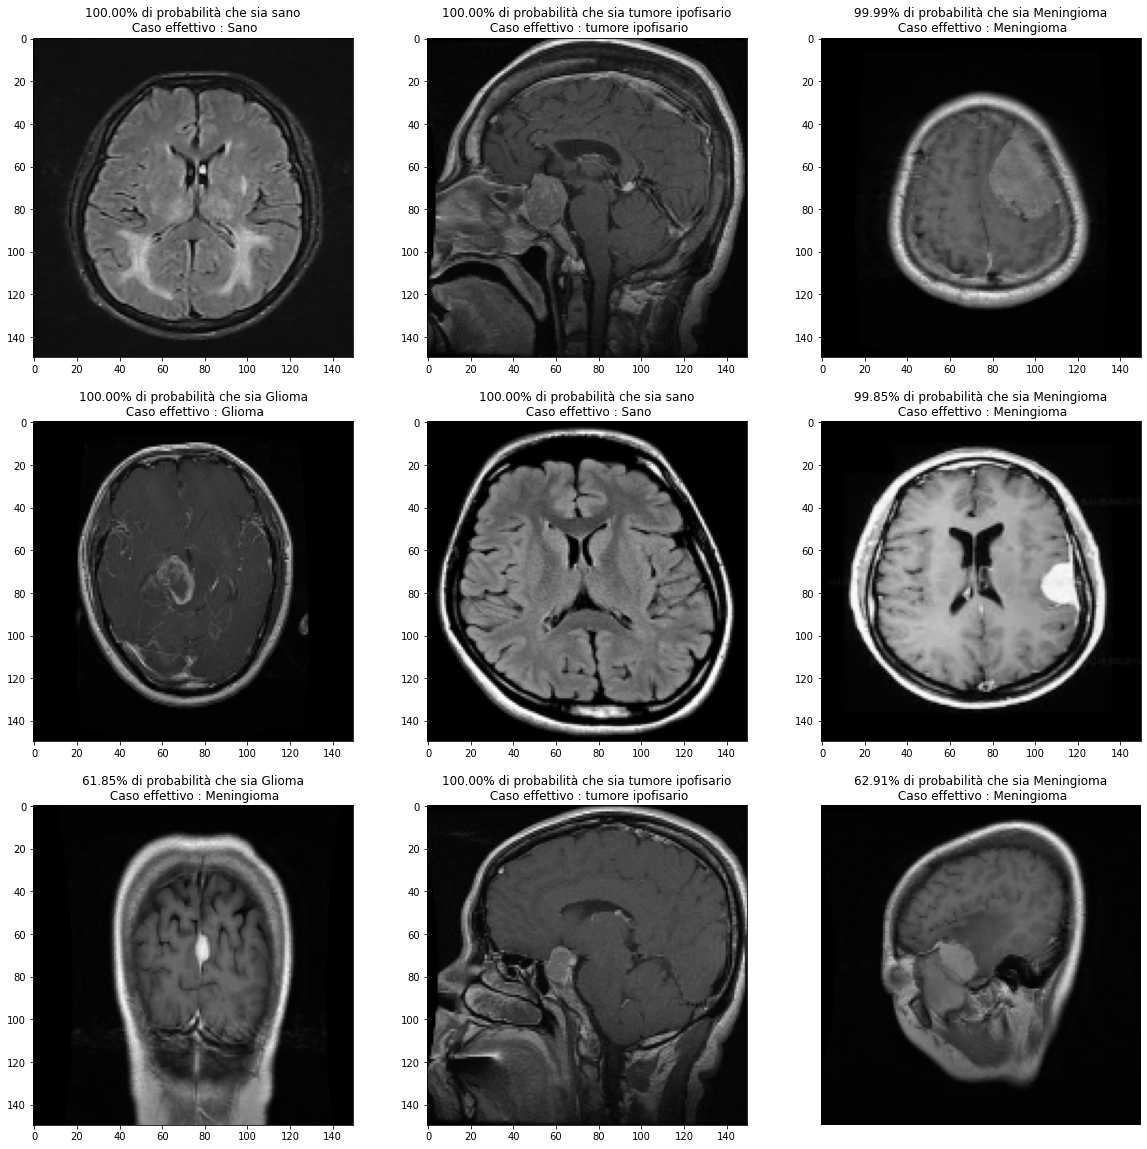
\includegraphics[width=1.1\textwidth]{Figures/brain-tumr-results.png}
        \caption{\small{Predizioni fatte dal modello con associata la relativa probabilità versus 
        quelle effettive su un insieme di immagini (codice di realizzazione nel capitolo 7).
        } % end small
        } % end caption
        \label{fi:dcalc}
      \end{figure}
    \newpage
    \subsection{Considerazioni finali}
    In tutti e 3 i casi si sono raggiunti risultati soddisfacenti, nonostante il dataset portasse con sè non poche difficoltà 
    per il suo numero limitato di immagini. Sicuramente
    a differenza del dataset della polmonite, in cui la classificazione era binaria e ciononostante erano a disposizione un maggior numero di esempi, 
    in questi casi in cui la classificazione è multiclasse la scelta migliore è andare a utilizzare un modello preesistente. \\
    Se si vogliono ottenere buoni risultati partendo da 0 è necessario un buon modello con un numero di parametri da allenare che 
    non sia troppo elevato (come nel caso del primo modello) se non si vuole impiegare troppo tempo nel training rispetto a quella che sono le effettive dimensioni dei dati e i risultati ottenuti, e che la scelta di come andare ad aggiungere rumore sia ben ponderata.
    Sono state fatte prove anche con \lstinline{image_size} pari a 224, perchè tale numero di pixel per le immagini di input era 
    risultato ottimale per AlexNet (vedasi paper del 2012 scritto dagli autori~\cite{alexnet}), e con \lstinline{batch_size} pari a 8, 32 e 64. \\
    Il valore del learning rate è stato regolato come nel caso della polmonite automaticamente grazie all'ottimizzatore Adam, 
    che parte da un valore di 0.01 e tramnte la funzione di riduzione del learning rate, si riescono a superare i momenti di 
    stagnazione dell'apprendimento uscendo al di fuori dei minimi locali della funzione di perdita. 
    Si riportano a titolo di esempio i risultati medi ottenuti per 5 training del primo modello al variare
     degli iperparametri, i quali hanno portato a definire quelli ottimali e di fare fine-tuning (stessa cosa è stata ripetuta con le altre architetture).
    \begin{center}
      
    \begin{table}
      \begin{tabular}{l|lll}
        
      \hline
                                                                                                         & \multicolumn{1}{l|}{\textbf{training accuracy}} & \multicolumn{1}{l|}{\textbf{validation accuracy} }\\ \hline
      \textbf{\begin{tabular}[c]{@{}l@{}}batch = 8\\ image size = 150x150\\ channels = 3\end{tabular}}  & 99.9\%                                         & 93.3\%                                          \\ \hline
      \textbf{\begin{tabular}[c]{@{}l@{}}batch = 32\\ image size = 150x150\\ channels = 3\end{tabular}}  & 99.9\%                                         & 93.4\%                                          \\ \hline
      \textbf{\begin{tabular}[c]{@{}l@{}}batch = 64\\ image size = 150 x 150\\ channels = 3\end{tabular}} & 98.9\%                                         & 80.7\%                                          \\ \hline
      \textbf{\begin{tabular}[c]{@{}l@{}}batch = 32\\ image size = 150 x 150\\ channels = 1\end{tabular}} &  99.7\%                                     &  91.3 \%                                       \\ \hline
      \textbf{\begin{tabular}[c]{@{}l@{}}batch = 8\\ image size = 224x224\\ channels = 3\end{tabular}}  & 99.9 \%                                         & 93.1\%                                          \\ \hline
      \textbf{\begin{tabular}[c]{@{}l@{}}batch = 32\\ image size = 224x224\\ channels = 3\end{tabular}}  & 99.8\%                                       &  93.2\%                                       \\ \hline
      \textbf{\begin{tabular}[c]{@{}l@{}}batch = 64\\ image size = 224 x 224\\ channels = 3\end{tabular}} & 99.9\%                                         & 93.1\%                                          \\ \hline
      \textbf{\begin{tabular}[c]{@{}l@{}}batch = 32\\ image size = 224 x 224\\ channels = 1\end{tabular}} &  99.8\%                                        &  92.7\%                                       \\ \hline
      \end{tabular}
      \caption{Si noti che tra tutti i training quello in cui si sono ottenuti i risultati in media migliori per il test è quello con gli iperparametri pari a quelli della seconda riga.}
   
      \end{table}

    \end{center}
 
